\documentclass[12pt,spanish,fleqn,openany,letterpaper,pagesize]{scrbook}

\usepackage[utf8]{inputenc}
\usepackage[spanish]{babel}%escribir con acentos sin necesidad de comandos \'{} .
\usepackage{fancyhdr}
\usepackage{epsfig}
\usepackage{epic}
\usepackage{eepic}
\usepackage{amsmath}
\usepackage{threeparttable}
\usepackage{amscd}
\usepackage{here}
\usepackage{graphicx}
\usepackage{lscape}
\usepackage{tabularx}
\usepackage{subfigure}
\usepackage{longtable}
\usepackage{multirow}
\usepackage[shortlabels]{enumitem}

\usepackage{rotating} %Para rotar texto, objetos y tablas seite. No se ve en DVI solo en PS. Seite 328 Hundebuch
                        %se usa junto con \rotate, \sidewidestable ....

\renewcommand{\theequation}{\thechapter-\arabic{equation}}
%\renewcommand{\thefigure}{\textbf{\thechapter-\arabic{figure}}}
\renewcommand{\thetable}{\textbf{\thechapter-\arabic{table}}}


\pagestyle{fancyplain}%\addtolength{\headwidth}{\marginparwidth}
\textheight22.5cm \topmargin0cm \textwidth16.5cm
\oddsidemargin0.5cm \evensidemargin-0.5cm%
\renewcommand{\chaptermark}[1]{\markboth{\thechapter\; #1}{}}
\renewcommand{\sectionmark}[1]{\markright{\thesection\; #1}}
\lhead[\fancyplain{}{\thepage}]{\fancyplain{}{\rightmark}}
\rhead[\fancyplain{}{\leftmark}]{\fancyplain{}{\thepage}}
\fancyfoot{}
\thispagestyle{fancy}%


\addtolength{\headwidth}{0cm}
\unitlength1mm %Define la unidad LE para Figuras
\mathindent0cm %Define la distancia de las formulas al texto,  fleqn las descentra
\marginparwidth0cm
\parindent0cm %Define la distancia de la primera linea de un parrafo a la margen

%Para tablas,  redefine el backschlash en tablas donde se define la posici\'{o}n del texto en las
%casillas (con \centering \raggedright o \raggedleft)
\newcommand{\PreserveBackslash}[1]{\let\temp=\\#1\let\\=\temp}
\let\PBS=\PreserveBackslash

%Espacio entre lineas
\renewcommand{\baselinestretch}{1.1}

%Neuer Befehl f\"{u}r die Tabelle Eigenschaften der Aktivkohlen
\newcommand{\arr}[1]{\raisebox{1.5ex}[0cm][0cm]{#1}}

%Neue Kommandos
\usepackage{Befehle}
%Inicio del documento. Tener en cuenta que hay archivos auxiliares

\begin{document}
\pagenumbering{roman}
%\newpage
%\setcounter{page}{1}
\begin{center}
\begin{figure}
\centering%
\epsfig{file=HojaTitulo/escudo,scale=0.65}
\end{figure}
\thispagestyle{empty} \vspace*{0cm} \textbf{\huge
Asociación de variantes en regiones codificantes de genes con datos clínicos en
pacientes colombianos usando minería de datos}\\[5.0cm]
\Large\textbf{Jennifer Vélez Segura}\\[5.0cm]
\small Universidad Nacional de Colombia\\
Facultad de Ingeniería, Departamento de Ing. Sistemas e Industrial\\
Bogotá D.C., Colombia\\
2019\\
\end{center}

\newpage{\pagestyle{empty}\cleardoublepage}

\newpage
\begin{center}
\thispagestyle{empty} \vspace*{0cm} \textbf{\huge
Asociación de variantes en regiones codificantes de genes con datos clínicos en
pacientes colombianos usando minería de datos}\\[2.0cm]
\Large\textbf{Jennifer Vélez Segura}\\[2.0cm]
\small Tesis presentada como requisito parcial para optar al
t\'{\i}tulo de:\\
\textbf{Magíster en Bioinformática}\\[2.5cm]
Director(a):\\
Ph.D. Elizabeth León Guzmán\\[2.0cm]
L\'{\i}nea de Investigaci\'{o}n:\\
Minería de datos en Bioinformática\\
Grupo de Investigaci\'{o}n:\\
MIDAS\\[2.5cm]
Universidad Nacional de Colombia\\
Facultad Ingeniería, Departamento de Ing. Sistemas e Industrial\\
Bogotá D.C., Colombia\\
2019 \\
\end{center}

\newpage{\pagestyle{empty}\cleardoublepage}

\newpage
\thispagestyle{empty} \textbf{}\normalsize
\\\\\\%
\textbf{(Dedicatoria)}\\[4.0cm]

\begin{flushright}
\begin{minipage}{8cm}
    \noindent
        Esta tesis esta dedicada a mi familia quienes han sido mi principal apoyo y soporte durante toda mi vida y a mi mejor amiga que en paz descanse Camila Marcela Sanchez Rubio.\\[1.0cm]\\
      \end{minipage}
\end{flushright}

\newpage{\pagestyle{empty}\cleardoublepage}

\newpage
\thispagestyle{empty} \textbf{}\normalsize
\\\\\\%
\textbf{\LARGE Agradecimientos}
\addcontentsline{toc}{chapter}{\numberline{}Agradecimientos}\\\\
A mis amigos Sergio Solano y Julián Cruz quienes me apoyaron, durante todo el proceso de desarrollo del trabajo, al laboratorio Genetix S.A.S quienes donaron la información utilizada en el presente trabajo, a mis compañeras del laboratorio,a mi familia por todo el apoyo y la paciencia.Finalmente a la profesora Elizabeth León Gúzman por la aceptar la dirección del trabajo y prestar todos sus conocimientos para la culminación de este trabajo. \\

\newpage{\pagestyle{empty}\cleardoublepage}

\newpage
\textbf{\LARGE Resumen}
\addcontentsline{toc}{chapter}{\numberline{}Resumen}\\\\
En esta tesis de maestría se propone un modelo para el análisis de variantes en regiones codificantes de genes con datos de pacientes colombianos usando técnicas de minería de datos. Para ello se implementó y valido un pipeline para la identificación de variantes Se realizó una implementación y validación de un pipeline para la identificación de variantes a partir de 4813 secuenciados de 227 pacientes colombianos, las variantes fueron prefiltradas según su calidad y almacenadas en una base de datos. Esta base de datos fue . Se diseño e implemento un modelo de datos para la gestión de la información de las variantes obtenidas y se le adiciono la información clínica disponible para 227 pacientes. Se diseño un modelo de minería de datos basados en procesamiento de lenguaje natural de las historias clínicas y las cuales se les realizo un agrupamiento, una vez obtenidas. \\

Se propuso un modelo para análisis textual de historias clínicas, y reglas de asociación para describir cada uno de los grupos encontrados y sus variantes. Adicionalmente se realizo un análisis puntual de asociación de variantes a los genes CFTR que es un gen con alta variabilidad y asociado a fibrosis quística  y el RB1 que es un gen de baja variabilidad que esta asociado a retinoblastoma infantil y a cáncer de hueso y de vejiga. Se obtuvieron 5 grupos de pacientes con diferentes variantes asociadas, mientras que para el gen CFTR se obtuvieron las variantes frecuentes de toda la población sin una asociación a la fibrosis quística, pero para RB1 si se obtuvieron variantes para retinoblastoma y como factores de riesgo en dos grupos distintos. El modelo permitió hacer una caracterización de la frecuencia de variantes en 227 pacientes y por cada uno de los grupos obtenidos.  \\

\textbf{\small Palabras clave: Secuenciación, variantes, región codificante, minería de datos, agrupamiento, reglas de asociación, modelo de datos, características clínicas}.\\


\textbf{\LARGE Abstract}\\\\
An implementation and validation of a pipeline was carried out to identify variants from 4813 sequenced. A data model for information management was designed and implemented. It is a data mining model in natural language processing of clinical histories and those that are grouped, once you get the groups apply the rules of association for each of the groups and the two genes that were  CFTR and RB1. The results were classified in the database, in the database and in the database. A mining model is implemented that allows to characterize and associate the frequency of the variants in the genes to the clinical characteristics of the patients.\\[2.0cm]
\textbf{\small Keywords: Sequencing, variants, coding region, data mining, clustering, association rules, information systems, clinical characteristics.}\\


\renewcommand{\tablename}{\textbf{Tabla}}
\renewcommand{\figurename}{\textbf{Figura}}
\renewcommand{\listtablename}{Lista de Tablas}
\renewcommand{\listfigurename}{Lista de Figuras}
\renewcommand{\contentsname}{Contenido}
\tableofcontents % indice de tablas


%\newcommand{\clearemptydoublepage}{\newpage{\pagestyle{empty}\cleardoublepage}}

%\include{Tab_Simbolos/TabSimbolosMSc}
%\include{Resumen}%\newcommand{\clearemptydoublepage}{\newpage{\pagestyle{empty}\cleardoublepage}}
\pagenumbering{arabic}
\cleardoublepage
\addcontentsline{toc}{chapter}{Lista de figuras} % para que aparezca en el indice de contenidos
\listoffigures % indice de figuras

\cleardoublepage
\addcontentsline{toc}{chapter}{Lista de tablas} % para que aparezca en el indice de contenidos
\listoftables % indice de tablas

\chapter{Estado del Arte}

\section{Biología molecular y secuenciación masiva.}

Desde  que  Watson y Crick propusieron la estructura del ADN en 1953 \cite{Watson1953}, el estudio del ADN ha sido básico en el desarrollo de la biología molecular, incluso el mismo Francis Crick fue quien propuso el dogma central de la misma para describir la relevancia del ADN en los seres vivos y la utilización de la información que contiene por las células,dada la importancia del  ADN  en las décadas de 1970 y 1980 se desarrollaron  técnicas para determinar el orden de los nucleótidos  (técnicas de secuenciación) de manera más eficiente que la secuenciación de las proteínas y se definieron secuencias de algunos organismos como el virus de Episten Barr y  de la mitocondria humana, mediante la utilización de métodos químicos propuestos por Maxam y Gilbert en 1977 y Sanger en 1980 siendo este último el más popular, estas técnicas son conocidas como tecnicas primera generación \cite{Herraez2012}. 

Los métodos desarrollados para secuenciar prosperaron y con el proyecto del genoma humano que comenzó en 1980 y fue completado en el 2003, permitió que se desarrollaran nuevas tecnologías para optimizar el proceso de secuenciación y disminuir sus costos, inicialmente fue el secuenciador de Illumina  que en el 2008 permitió obtener el primer individuo humano secuenciado con esta tecnología [3]. Estas nuevas tecnologías se fueron desarrollando en otras plataformas, tales como el secuenciador de roche 454, y el SOLiD de applied biosisten [3] y son conocidas como tecnologías de última generación o de siguiente generación (Next-generation sequencing, NGS), que tienen la capacidad de realizar secuenciaciones de alto rendimiento de una maneras más rápida y económica que las de primera generación [2]. La diferencia entre las técnicas de secuenciación de primera generación y las de NGS se presenta en el hecho de que la nueva generación genera lecturas de menos de 500 pares de bases en comparación a las 1000 pares de bases [3]. 

El desarrollo de estas tecnologías ha hecho que los datos biológicos aumenten de una manera vertiginosa, y permiten que se pueda realizar análisis de genómicos de diferentes organismos, análisis de ARN, que permiten aplicaciones en biotecnología y salud [4]. En el campo de la salud actualmente se emplea la secuenciación de exomas principalmente puesto que se considera que los exones son las regiones de ADN conservadas y expresadas, (se traducirán en ARNm y posteriormente en proteínas) y representan menos del 2% el genoma humano pero se estima que contiene el 85% de las variantes conocidas de enfermedades, lo que permite la reducción de costos y una buena alternativa frente a la secuenciación de genomas completos [5] [6]. 

La secuenciación de exones (secuenciación de exoma) ha sido un buen método para identificar SNPs (Polimorfismos de Nucleótido Único), y permitió identificar pequeñas delecciones o inserciones (indels) que pueden  ser la causa de enfermedades y de la variación en los fenotipos [7]. MiSeq es un sistema de secuenciación de illumina que permite la secuenciación de 4800 genes en un solo experimento [6]. En cuanto al análisis de los datos esta plataforma incluye un servició de computación en la nube (BaseSpace), donde los datos biológicos son analizados  sin necesidad de que los investigadores tengan habilidades en bioinformática. Pero están disponibles como herramientas solamente de investigación y no como diagnóstico [8] . 

A pesar de ser herramientas de investigación  que han sido desarrolladas, Illumina permite que dentro del BaseSpace se publiquen nuevos algoritmos, herramientas abiertas o aplicaciones diseñadas por desarrolladores que permitan mejorar estos análisis genómicos y con la aplicación en diversas plataformas de secuenciación que ofrece esta empresa [9].

Los datos obtenidos a partir de técnicas de NGS han tenido un crecimiento vertiginoso y presentan un reto para el manejo y análisis de los mismos, debido a que los formatos de los datos y las inconsistencias de las secuencias como resultado de los procesos experimentales, la importación de las secuencias a nivel digital, el ensamble de los fragmentos de ADN, el alineamiento y post-alineamiento de grandes cantidades de datos biológicos hace que se convierta en una de las bases de la investigación en bioinformática [7] [10].

Datos biológicos como “big data”.

En la era de las omícas, los datos se presentan en diferentes formas y en varios niveles en términos biológicos, los cuales incluyen los datos genómicos, datos de transcriptomica, epigenomica, metabulomica, entre otros, donde se incluyen también las diferentes datos poblacionales humanos y las historias clínicas, la escala de estos datos se encuentran  entre  pentabyte y exabyte [11]. La definición de “big data” es muy discutido dentro de las ciencias de la información, sin embargo el nombre  hace referencia a la “gran cantidad de datos” que se caracterizan por el volumen del procesamiento, la variabilidad de los mismos y la veracidad de la calidad de los datos [11]. Partiendo de lo anterior los datos biologícos pueden ser catalogados como “big data” ya que poseen las siguientes características: Son numerosos, no pueden ser almacenados dentro de una base regular de datos, la velocidad  de generación y procesamiento es muy rápida [12].

Para el manejo de los datos se han aplicado varios modelos de sistemas de información en  bioinformática con diversas herramientas para integrar datos biológicos, utilizando sistemas de bodega de datos que están disponibles de manera gratuita y que fueron desarrollados con el fin de dar respuesta algunos de los problemas en el manejo de datos biológicos, dada la importancia que tiene de poder utilizar toda la información necesaria de manera eficiente [10]. En la tabla 1 se describen algunos softwares libres para la integración de datos:

\chapter{Introducci\'{o}n}

El desarrollo de este trabajo responde a la necesidad actual del país en cuanto a la utilización las nuevas tecnologías de secuenciación masiva aplicadas a la salud de los colombianos, cuyos aportes muestran la relevancia del uso de estas tecnologías en el país que al ser combinadas con métodos de análisis de datos a gran escala permitiendo mostrar un acercamiento de la estructura genética de la población colombiana asociada a la información clínica disponible de los participantes dentro del estudio.\\

Además de mostrar la importancia de que exista una relación estrecha entre ciencia y tecnología para mejorar el diagnóstico y pronostico de enfermedades presentes en la población colombiana aprovechando todas las avances que se encuentran a disposición actualmente y que permiten generar nuevos aportes con un impacto real en la salud.\\

En los últimos años con el desarrollo de las tecnologías NGS (Secuencieción de siguiente generación o secuenciación masiva) y otras áreas de la informática se ha introducido una nueva área en las tecnologías de la información conocida como Big Data \cite{Mohammed2014}. En el campo de la bioinformática en concreto es el exoma o secuenciación del genoma completo (WES o WGS), que generan una gran cantidad de información con diferentes aplicaciones en la biotecnología y en la  salud de nivel mundial \cite{Hwang2015}. La enorme cantidad de datos obtenidos por estas nuevas tecnologías presentan son una desafío para ser analizados dado que la estadística tradicional aplicada en genética es poco efectiva para analizar datos de secuenciación de exomas y genomas debido a la gran cantidad de variantes que se obtienen a partir de los experimentos de secuenciación \cite{Wu2014,Mohammed2014}.\\

La aplicación de la secuenciación masiva es posible de aplicar gracias a  la reducción de costos y por su capacidad para dar un dar un posible diagnóstico a pacientes que se les sospecha de un síndrome genético de características ambiguas y que con otros estudios no es posible aclarar, o para ser aplicados en paneles genéticos a pacientes que se les sospecha un síndrome especifico \cite{Hegde2017}.\\

Los datos biológicos en la actualidad están en la escala de petabyte y exabyte,presentando el reto de integrar información  y de realizar su posterior análisis, por lo tanto es necesario desarrollar sistemas de información para el manejo y consulta de los datos obtenidos donde los genotipos y los fenotipos,dado que los datos de secuenciación contienen grandes cantidades de información que usualmente se almacena en bases de datos relacionales, después de realizada la anotación de variantes \cite{Li2014} \cite{Lauzon2016}.\\

Estos datos son considerados como "big data" \ dado que cumplen con los criterios de grandes cantidades de información, velocidad de procesamiento y veracidad de los datos, un ejemplo de esto fue el proyecto de 1000 Genomas, el cual por medio de la secuenciación de genomas completos se genero un sistema de información pública que contiene aproximadamente tres billones de nucleótidos y en el cual la población colombiana no esta correctamente representada dado que se tomo solo una muestra poblacional de la ciudad de Medellín. Además estudios como el perfil de BRCA1 y BRCA2 con la implementación de la secuenciación masiva no tampoco representa la población  colombiana\cite{Li2014,CoriellInstitute,Arias-blanco2015}.\\
 
La importancia de la caracterización de la población colombiana esta dada porque la frecuencias de las variantes tienen un alto impacto en la clasificación de la misma siendo las variantes con baja frecuencia poblacional como posibles variantes patogénicas según la ACGM (Asociación Americana de Genética Médica)\cite{Li2017}.\\

Para el manejo de estos tipos de datos se han desarrollado diversas herramientas que incluyen el procesamiento computacional y gestión de estos tipos de datos, así como la creación de buenas prácticas en marco de la integración del análisis de una manera reproducible. Pero el manejo de esta informaci\'on por parte de los profesionales de las ciencias biol\'igicos es una gran limitante dado que no tienen fundamentos de programacio\'in ni conocen los procedimientos que se utilizan normalmente en las ciencias de la computacio\'n, por lo tanto prefiren utilizar herramientas ma\'s amigables para su uso, pero esto implica un lento procesamiento de los datos ya que los flujos de trabajo que se lleguen a desarrollar son mediante aplicaciones gra\'ficas que consumen ma\'s recursos computacionales \cite{Fisch2015}.\\

La gestión y análisis de esta información requiere el desarrollo de herramientas que respondan a las necesidades de obtener características relevantes de la información biológica, por ello la implantación de técnicas minería de datos permiten generar hipótesis especificas con respecto a la información genómica \cite{Huttenhower2010}. Un ejemplo de esto es la utilización de algoritmos de agrupamiento para encontras grupos de genes que están fuertemente relacionados con estados de evolución de los diferentes estadios en cáncer \cite{Li2014}.\\

La gran cantidad de datos biológicos que se encuentran disponibles en la actualidad, deben ser tenidos en cuenta para la investigación y  uso en el diagnóstico clínico, sin embargo estos datos presentan los siguientes inconvenientes para su acceso y disponibilidad como son: el almacenamiento, el procesamiento, la conexión y el análisis integrado de los mismos \cite{Pabinger2014}. Por esta razón, en los procesos de diagnóstico se hace necesario reconocer los patrones  sintomáticos de pacientes de los pacientes y asociarlos con variantes genéticas, ya que no ha sido posible realizarlo fácilmente por diversas causas como la perdida de información relevante el acceso a la misma, por ejemplo los datos que reposan en las historias clínicas, que para su acceso se requiere solicitar un permiso \cite{Pabinger2014}. \\

La importancia de entender las formas genéticas que pueden causar diversos síndromes y patología, pueden permitir que se le dé prioridad diagnostica y de tratamiento a los pacientes afectados, teniendo en cuenta que aún se continua descubriendo nuevos genes asociados a enfermedades, teniendo en cuenta que existen retos computacionales como la integración de datos heterogéneos y de grandes cantidades que lleva a la necesidad de aplicar metodologías “big data” y minería de datos para análisis de datos génomicos \cite{Maharjan2011,Hannah-Shmouni2015,Louie2007}. La diversidad de los datos permite que la utilización de técnicas de minería de datos se pueda aprovechar para dar respuesta al problema de asociación entre variantes genéticas y el impacto clínico de esas variantes \cite{Pabinger2014}.
\\

En el presente trabajo se desarrollaron las siguientes actividades:

\begin{enumerate}  
	\item La implementación y validación de un pipeline para la identificación de variantes.
	\item El diseño e implementación de un sistema de información para realizar la gestión de datos para las variantes obtenidas junto con la información clínica.
	\item Finalmente un modelo para la  minería de datos aplicada en pacientes colombianos.
\end{enumerate}
 
\section*{Objetivos}

\subsection*{Objetivo General}%* para sileciar el capitulo en la tabla de contenido.

Proponer un modelo de miner\'ia de datos para la identificaci\'on de variantes en regiones codificantes de genes  que apoyen el  diagn\'ostico cl\'inico en pacientes colombianos usando t\'enicas de miner\'ia de datos.


\subsection*{Objetivos Espec\'ificos}

\begin{enumerate}
	\item Generar un modelo de datos que permita la integraci\'on de los datos biol\'ogicos de tipo experimental, te\'orico y cl\'inicos en una  muestra poblacional que realice consultas r\'apidas de los datos almacenados.
	\item Dise\~nar un modelo de miner\'ia de datos permita identificar las variantes experimentales que puedan ser patog\'enicas, teniendo en cuenta par\'ametros de asociaci\'on entre genes e informaci\'on cl\'inica que posibiliten teorizar posibles predicciones de las variantes. 
	\item Implementar un  modelo de miner\'ia de datos que permita identificar posibles variantes patog\'enicas diferencialmente de las variantes no relevantes y  su asociaci\'on a la informaci\'on cl\'nica disponible.
	\item Validar el modelo de miner\'ia de datos implementado para la identificaci\'on de variantes patog\'enicas en pacientes colombianos utilizando regiones codificantes de genes asociados.  
\end{enumerate}

\section*{Contribuciones}

\begin{itemize}
	\item[$*$] Validación de un pipeline para la identificación de variantes en exomas humanos. Presentado en el Congreso de Genética Humana.2016
	\item[$*$] Diseño e implementación de la base de datos para integrar exomas ELAG.2017
	\item[$*$] Modelo de minería para análisis de variantes.
	\item[$*$] Estructura poblacional en una muestra de pacientes poblacionales.
\end{itemize}

\section*{Tesis Online}

El presente trabajo se distribuye en los capitulo de estado del arte, validación del pipeline para el análisis de variantes, diseño e implementación de una base de datos, modelo de minería dentro de la base de datos, conclusiones y trabajo futuro.


\chapter{Valiadación de un pipeline para la identificación de variantes}

En este capitulo se presenta el proceso para validar un pipeline que permitió la  identificación de variantes a partir de datos de secuenciación de siguientes generación (NGS), donde se utiliza datos públicos un paciente  para validar la calidad  de las variantes.

\section{Identificación de variantes}

Los pipelines son un componente integral de la secuenciación de siguiente generación (NGS), para el procesamiento de los datos en bruto y detectar las alteraciones genómicas que tienen un impacto en la salud de un paciente, por lo tanto se hace necesario desarrollo, validación y monitoreo de los pipelines son necesarios para disminuir los errores de la identificación de variantes ya que pueden tener una consecuencia negativa en la salud de los pacientes \cite{Roy2018}.

\subsection{Analisis Bioinformático de datos de secuenciación}

Los pipelines bioinformaticos para NGS son comumente desarollados en una plataforma especifica y pueden ser adaptados según las necesidades del laboratorio, la mayoría de los pipelines consisten en los siguientes pasos \cite{Roy2018}:

\begin{enumerate}[1.]
	\item Generación de secuencias.
	\item Alineamiento de las secuencias.
	\item Llamado de variantes.
	\item Filtrado de variantes.
	\item Anotación de variantes.
	\item Priorización de variantes. 
\end{enumerate}
 

La eficiencia de la identificación de variantes depende de la exactitud del llamado de las bases (la identificación correcta de cada nucleótido dentro de la secuencia), esto es realizado durante el proceso de secuenciación de alta velocidad con la que se identifican los nucleótidos hace que puedan ocurrir errores en la identificación correcta de las bases, se considera que al momento la exactitud de ese llamado esta alrededor del 99.5\% \cite{Tetreault2015}.Teniendo en cuenta lo anterior es recomendable  priorizar la sensibilidad (Buscar tantas variantes como sea posible para evitar perder cualquier variante) sobre la especificidad (Limita la proporción de falsos positivos en un conjunto de variantes) \cite{Auwera2014}.  \\

Para el presente trabajo se realizaron mediciones de la calidad de las secuencias y el mapeo, post-alineamiento y el llamado de variantes, siguiendo las buenas practicas para el llamado de variantes \cite{Fisch2015}.Teniendo en cuenta que existen múltiples herramientas para realizar el llamado de variantes tanto de uso privado como open source que permite  seguir las buenas practicas de identificación de variantes se hace necesario integrar las diversas herramientas para poder obtener las datos de buena calidad. Y surge la pregunta de ¿cuáles de todos los métodos y las herramientas son la más apropiada para hacer el llamado de variantes en exones \cite{Bao2014}\cite{Cornish2015}.\\

Para dar respuesta a esta pregunta se han seguido la propuesta de buenas practicas para el llamado de variantes propuesto por el Broad Institute que incluyen el procesamiento de los datos,el mapeo (Alinemaiento de las secuencias),descubrimiento de variantes y la recalibración del set de variantes.

Para poder llevar acabo la adecuada implementación se hace necesario la utilización de HPC (Computación de alto desempeño) donde la utilización de un clúster para bioinformática presentan una gran apoyo para el procesamiento y análisis de datos incluso es un requisito de algunos módulos para poder implementarse adecuadamente \cite{Fisch2015}.

\section{Datos}

Los datos que fueron procesados en el presente trabajo son secuencias de 4813 exones humanos se obtuvieron de kit de Illumina TruSight One en muestras de sangre periférica. Estos datos  fueron donados por el Centro de Investigaciones en Genética Humana y Reproductiva GENETIX S.A.S dirigido por la Dra Claudia Serrano Médico Genetista. \\

Para la validación del pipilene se corrio un exoma público de  NA12878-NGv3-LAB1360 que pertenece a una mujer que tiene una variación en el gen CYP2C19 donde tiene una transición de una Guanina por una Adenina en la posición 681 del exón 5, que causa un cambio en el marco de lectura del ARNm a partir del aminoácido 215 y produce un códon de parada prematuro en 20 aminoácidos corriente abajo produciendo una proteína no funcional (\textit{Información obtenida de Coriell Institute for medical reseach}). Se descargo el archivo bed para filtrar las variantes que se encuentran dentro del genoma completo de la muestra para obtener solo exones del NCBI para el genoma hg19.También se realizo una obtención de variantes a partir de un exoma completo público de la muestra NA12878,los datos fueron obtenidos via ftp en la siguiente direcciones:\\
\\
{\texttt{ https://s3.amazonaws.com/bcbio\_nextgen/NA12878-NGv3-LAB1360-A\_1.fastq.gz}\\
\\
{\texttt{ https://s3.amazonaws.com/bcbio\_nextgen/NA12878-NGv3-LAB1360-A\_2.fastq.gz}}\\
\\
Y el archivo bed para filtrar las variantes que se encuentran dentro del genoma completo de la muestra se obtuvo de la siguiente pagina para el genoma hg19: \\
\\
\texttt{ftp://ftp-trace.ncbi.nlm.nih.gov/giab/ftp/data/NA12878/analysis/}\\
\\
\texttt{Illumina\_PlatinumGenomes \_NA12877\_NA12878\_09162015/hg19/8.0.1/NA12878/} 

\section{Estrategias del pipeline}

Existen una serie de pasos para la obtención de variantes la obtención de la calidad de las secuencias y preprocesamiento como la remoción de adaptadores y de nucleótidos con baja calidad (que son erroneamente identificados por el secuenciador),posteriormente sigue el mapeo, post-alineamiento, llamado de variantes, anotación y priorización \cite{Bao2014}.\\

Se utilizo como base modulo de omics-pipe propuesto por Fish y colaboradores \cite{Fisch2015} que presenta el pipeline que es acorde con las buenas practicas para el llamado de variantes en la figura \ref{fig:pipeline}
	
\begin{figure}[] 
	\centering
	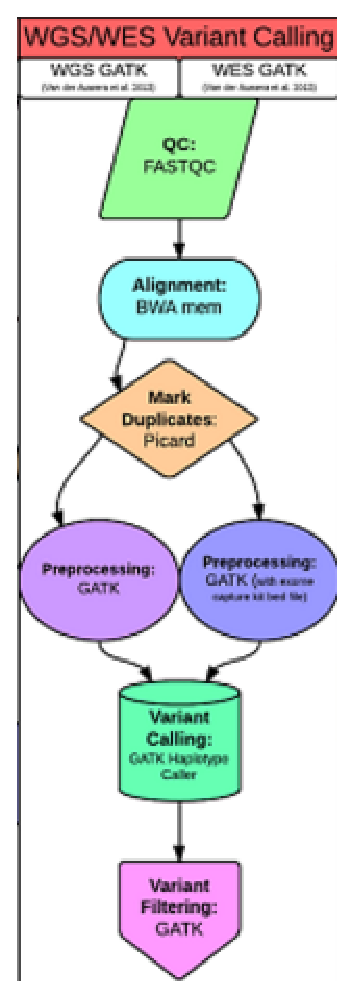
\includegraphics[width=0.2\textwidth]{Kap2/pipe}
	\caption{Pipeline basado en las buenas practicas para el llamado de variantes.} \label{fig:pipeline}
\end{figure}

Para el presente trabajo se adiciono el filtrado especifico de variantes según GATK y la parte de anotación de variantes con wAnnovar de la siguiente manera como muestra la siguiente figura \ref{fig:pipeline2}:

\begin{figure}[H] 
	\centering
	\includegraphics[width=0.6\textwidth]{Kap2/pipeline1}
	\caption{Pipeline basado en las buenas practicas para el llamado de variantes.} \label{fig:pipeline2}
\end{figure}
	
	\subsection*{Herramientas computacionales}
	
	Las herramientas bioinformáticas seleccionadas se implementaron en un clúster \footnote{El clúster utilizado fue prestado por la Universidad de los Andes} que cuenta con las siguientes características:
	
	\begin{itemize}
		\item[$\Rightarrow$] Un nodo mastes con 2 procesadores Intel Xeon E5-2695 – 24 cores 48 con HT / 192 GB RAM (230Gflops), 300 GB de Disco duro.
		\item[$\Rightarrow$] Se tienen 19 nodos de trabajo con 2 procecesadores  Intel Xeon E5-2695 – 24 cores 48 con HT / 192 GB RAM (4.378Tflops), 300 GB de de Disco duro.
		\item[$\Rightarrow$] Se cuentan con otros 7 nodos de trabajo con 4 procesadores AMD Opteron 6282 SE – 64 cores / 128 GB RAM (3.659Tflops), 200 GB de Disco duro.
		
		\item[$\Rightarrow$] 1 GPU tesla K20 como nodo de trabajo con 2 Procesores  Intel Xeon X5690 - 12 cores / 192 GB RAM (3.659Tflops), 1.6 TB de Disco duro.
		
	\end{itemize}
	
	Y se instalo el modulo para python de omics-pipe, para python 2 con la herramienta de R y las librerías que solicita omics-pipe\cite{Fisch2015} , el algoritmo BWA, samtools,vcftools, GATK 3.5,picard, FASTQC y pbs-drmma.Una vez instalados los programas se procesaron las muestras dentro del clúster.  

\subsection*{Diseños experimentales}

La tabla \ref{tabla:exp} muestra los diseños experimentales realizados para validar las variantes:

\begin{table}[htb]
	\begin{tabular}{|l|l|l|l|l|}
		\hline
		& \multicolumn{2}{c|}{\textbf{Experimentos}} \\
		\cline{2-3} 
		& NA12878(Exoma público)  & Variantes Illumina (Paciente)  \\ \cline{2-3}
		\hline 
		\multirow{1}{4cm}{Variantes Omics} & Datos de pacientes & Datos exoma   \\ \cline{2-3}
		\hline 
		\multirow{1}{4cm}{Variantes Calibradas} & Datos de paciente & Datos exoma    \\ \cline{2-3}
		\hline
		\multirow{1}{4cm}{Variantes Illumina} & Datos de paciente & Datos exoma     \\ \cline{2-3}
		\hline
	\end{tabular}
	\caption{Tabla de datos utilizados.}
	\label{tabla:exp}
\end{table}

\section{Resultados}
	\subsection*{Reporte FASTQC}}

Este reporte utilizando la herramienta FASTQC presenta inicialmente un resumen del estado de las secuencias obtenidas, ya que toma el archivo fastq y lee las métricas de calidad de cada una de las bases y genera un reporte general en formato HTML. Ya que es interactivo y genera varios módulos \cite{Babraham2016}. \\

Este reporte no presenta fallas dentro del análisis. A continuación se muestra un el primer modulo del reporte FASTQ obtenido de un dato experimental de una secuenciación de 4813 genes que resume el estado general de las lecturas obtenidas para este caso, la figura \ref{fig:fastq2} muestra que la calidad de las secuencias es mayor a 30, el reporte general también muestra que no hay secuencias adaptadoras, que presenta una distribución media del largo de las secuencias aceptable y que no hay secuencias sobre representadas.  \\

\begin{figure}[H]
	\centering
	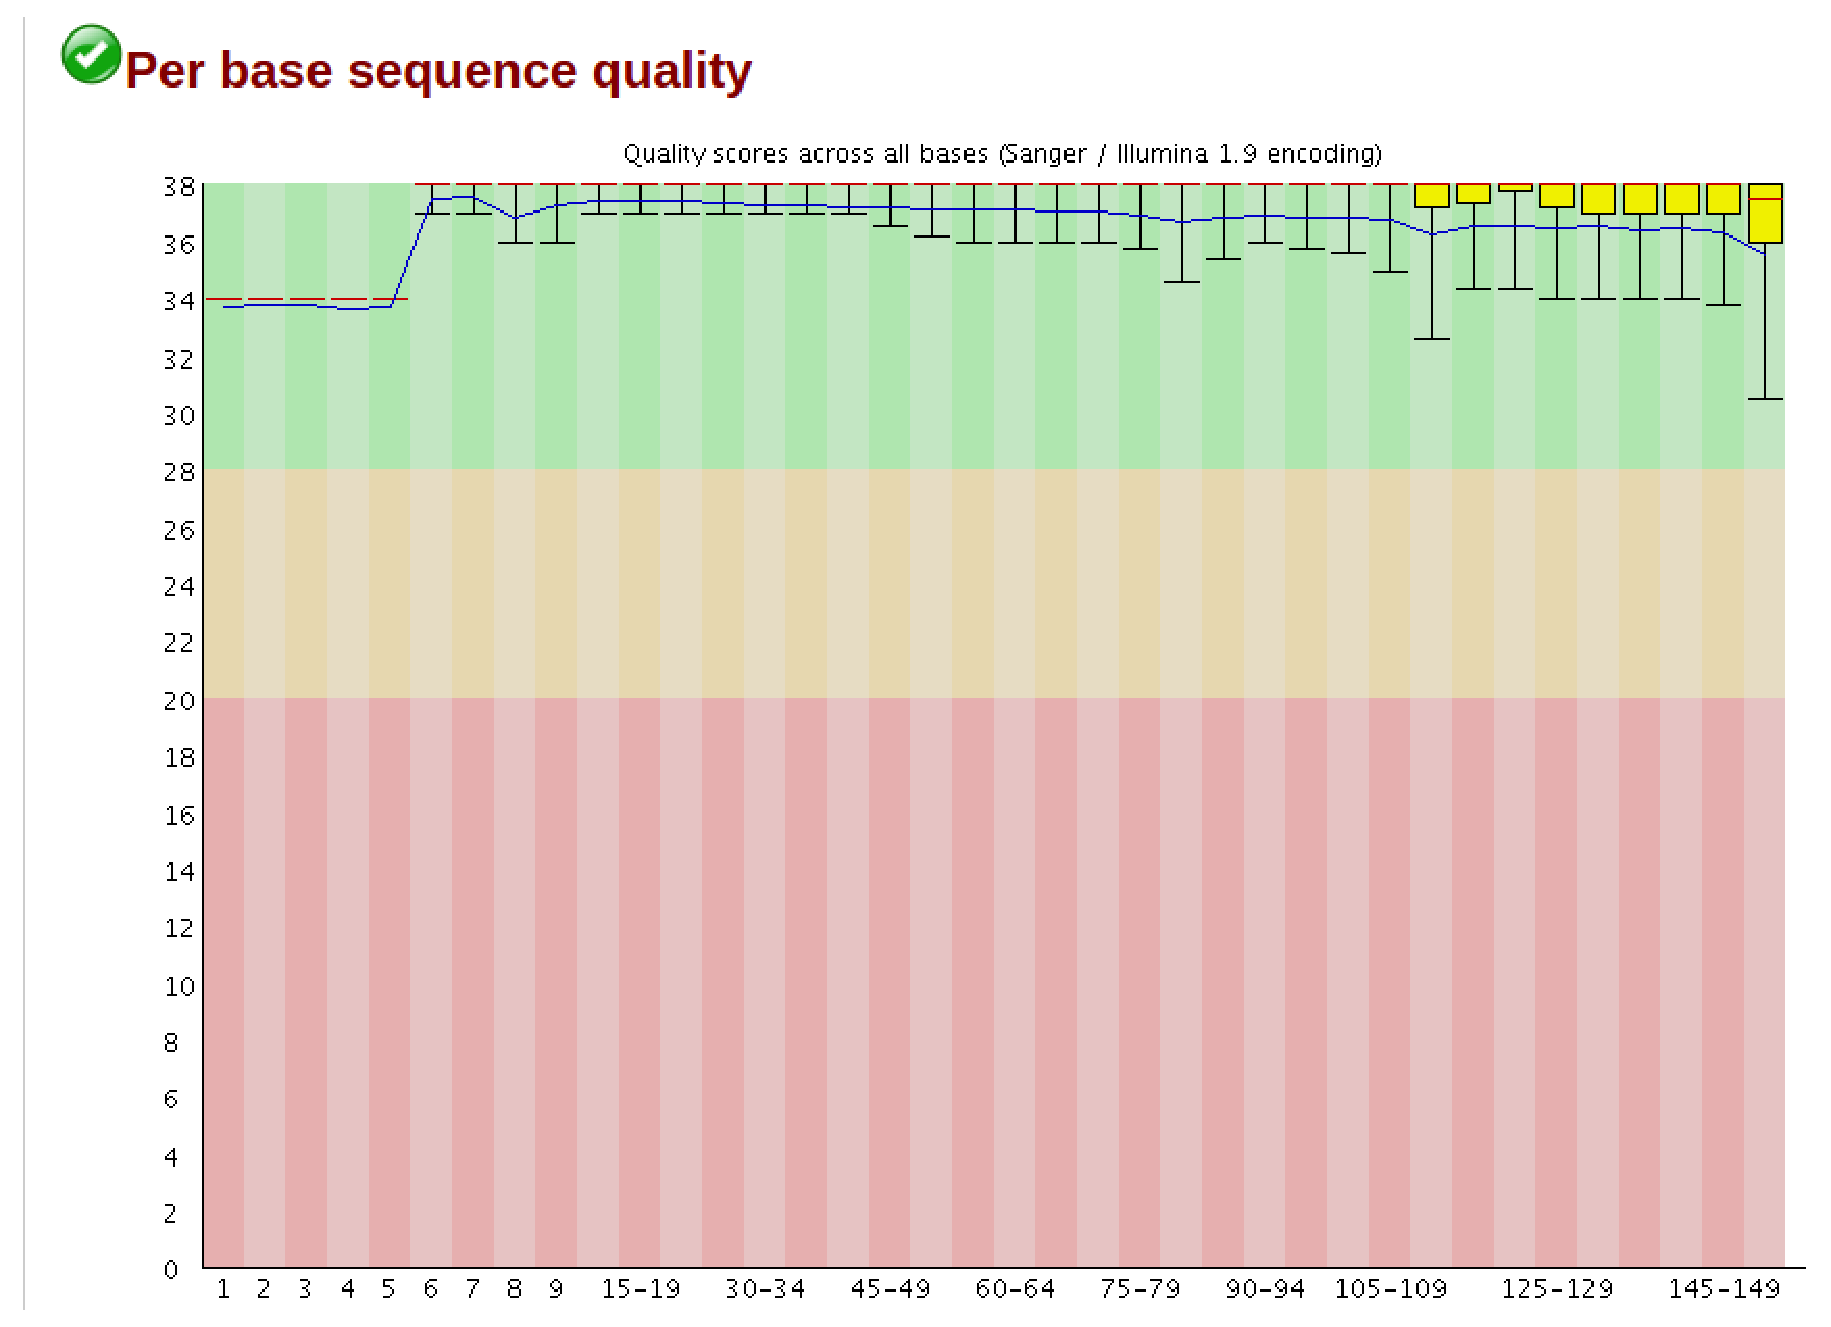
\includegraphics[width=0.4\textwidth]{Kap2/fastq2}
	\caption{Calidad del llamado de bases en una secuencia Estadísticas básicas del reporte FASTQ} \label{fig:fastq2}
\end{figure}

Para el caso de esta muestra la calidad es óptima en todos los datos obtenidos y no requieren de ningún tipo de trimming ya que la mayoría de las posiciones dentro de la secuencia se encuentran por encima del un valor por encima de 34 y el cual el valor mínimo es 20 (este valor representa el ($Q_{PHARED}$) que implementa el secuenciador \cite{Babraham2016}. \\ 

\subsection*{Variantes de illumina vs variantes de omics}

Inicialmente se obtuvieron 63515 variantes una vez que se ejecuto el pipeline de omics para la obtención de variantes, siguiendo los protocolos de buenas practicas y los protocolos de GATK quienes recomiendan generar variantes altamente sensibles y poco precisas, esto con el fin de no perder variantes que se encuentren dentro de las secuencias obtenidas, por ello se muestra una gran cantidad de variantes que no corresponden con las variantes verdaderas \cite{Auwera2014}.Dentro del pipeline solo se encuentra el proceso de llamado de variantes y no el proceso de filtrado de las mismas y que debío ser implementado de manera manual.\\

A partir de la aplicación del pipeline se obtuvieron los siguientes resultados representado en tabla (\ref{tabla:final}):

\begin{table}[htb]
	\centering
	\begin{tabular}{|l|l|l|l|l|}
		\hline
		& \multicolumn{4}{c|}{\textbf{Variantes}} \\
		\cline{2-5} 
		& SNP  & Indels & Desconocida & Total \\ \cline{2-5}
		\hline 
		\multirow{1}{4cm}{Variantes Omics} & 54538 & 8855 & 122 & 63515 \\ \cline{2-5}
		\hline 
		\multirow{1}{4cm}{Variantes Calibradas} & 10425 & 828 & 44 & 11297 \\ \cline{2-5}
		\hline
		\multirow{1}{4cm}{Variantes Illumina} & 9601 & 436 & 28 & 10065 \\ \cline{2-5}
		\hline
	\end{tabular}
	\caption{Tabla de Variantes obtenidas.}
	\label{tabla:final}
\end{table}

De las variantes sin hard filtering se obtuvieron 54538 SNP, Indels 8855 y 122 variantes desconocidas, que se representan el siguiente gráfico \ref{fig:omics}: 

\begin{figure}[H]
	\centering
	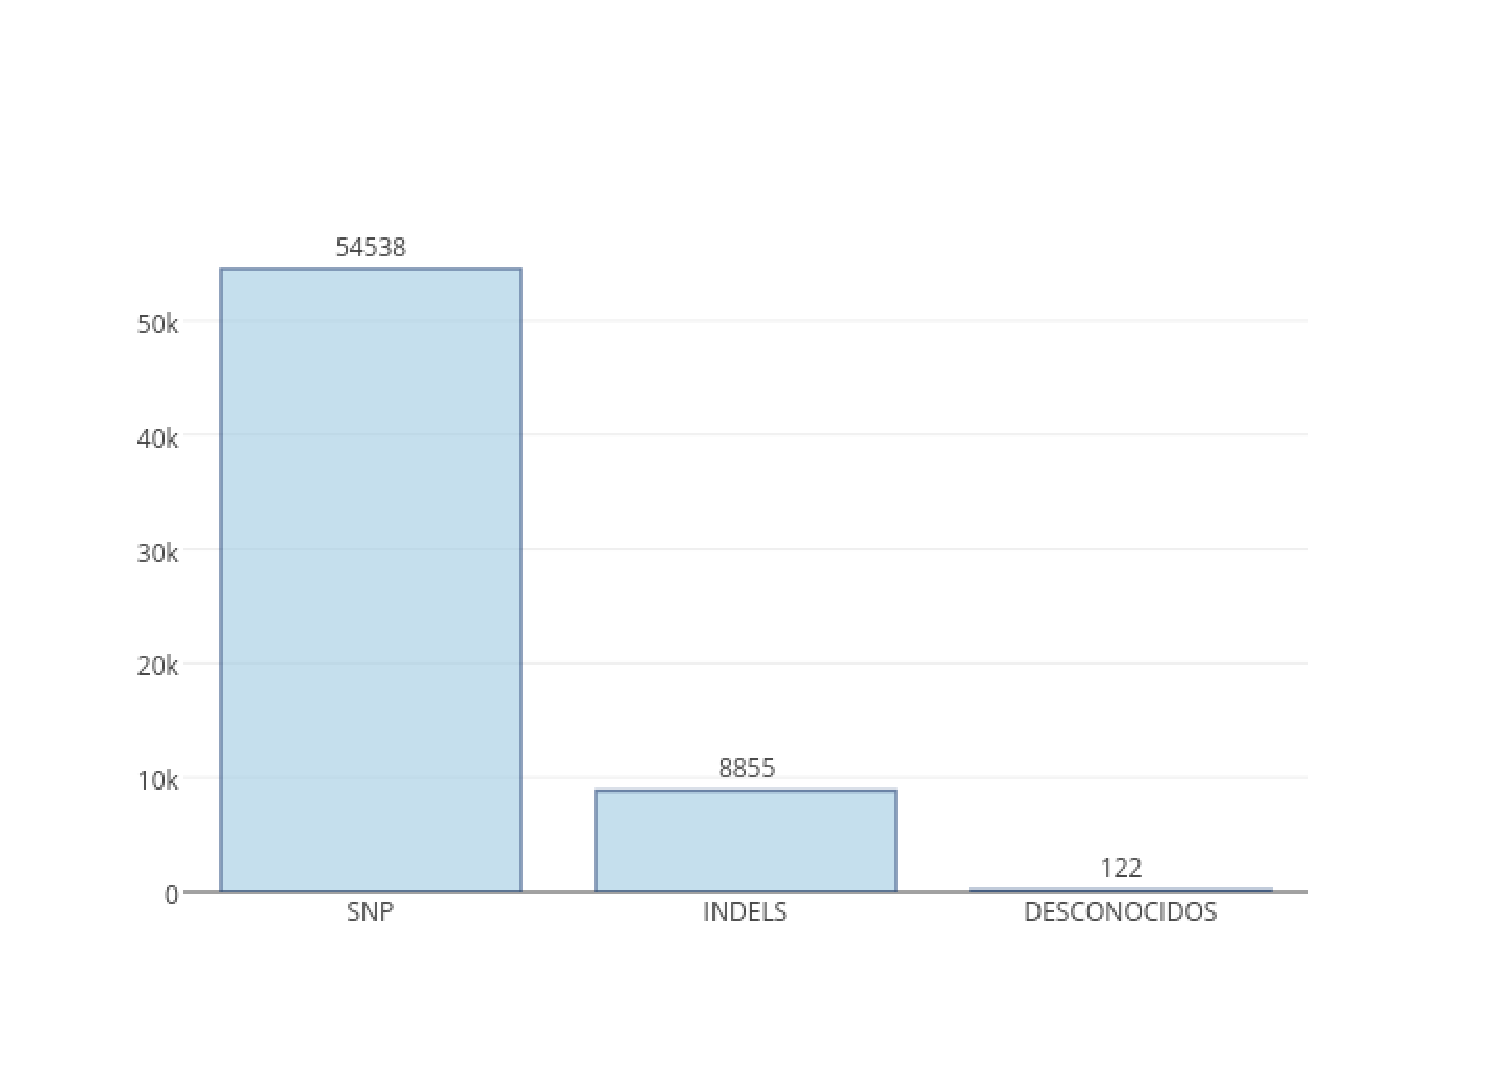
\includegraphics[width=0.5\textwidth]{Kap2/variantesomics}
	\caption{Variantes obtenidas por Omics pipe} \label{fig:omics}
\end{figure}

Una vez realizado el hard filtering se obtuvo los siguientes resultados: 10425 SNP, 828 Indels y 44 desconocidos, también se tiene las variantes reportadas para el mismo individuo desde la plataforma de illumina con los siguientes resultados: 9601 variantes, 436 indels y 28 desconocidas  y respresentado por la figura \ref{f:histogramas}:

\begin{figure}[H]
	\subfigure[Variantes obtenidas por Omics pipe]{
		\label{f:omics}
		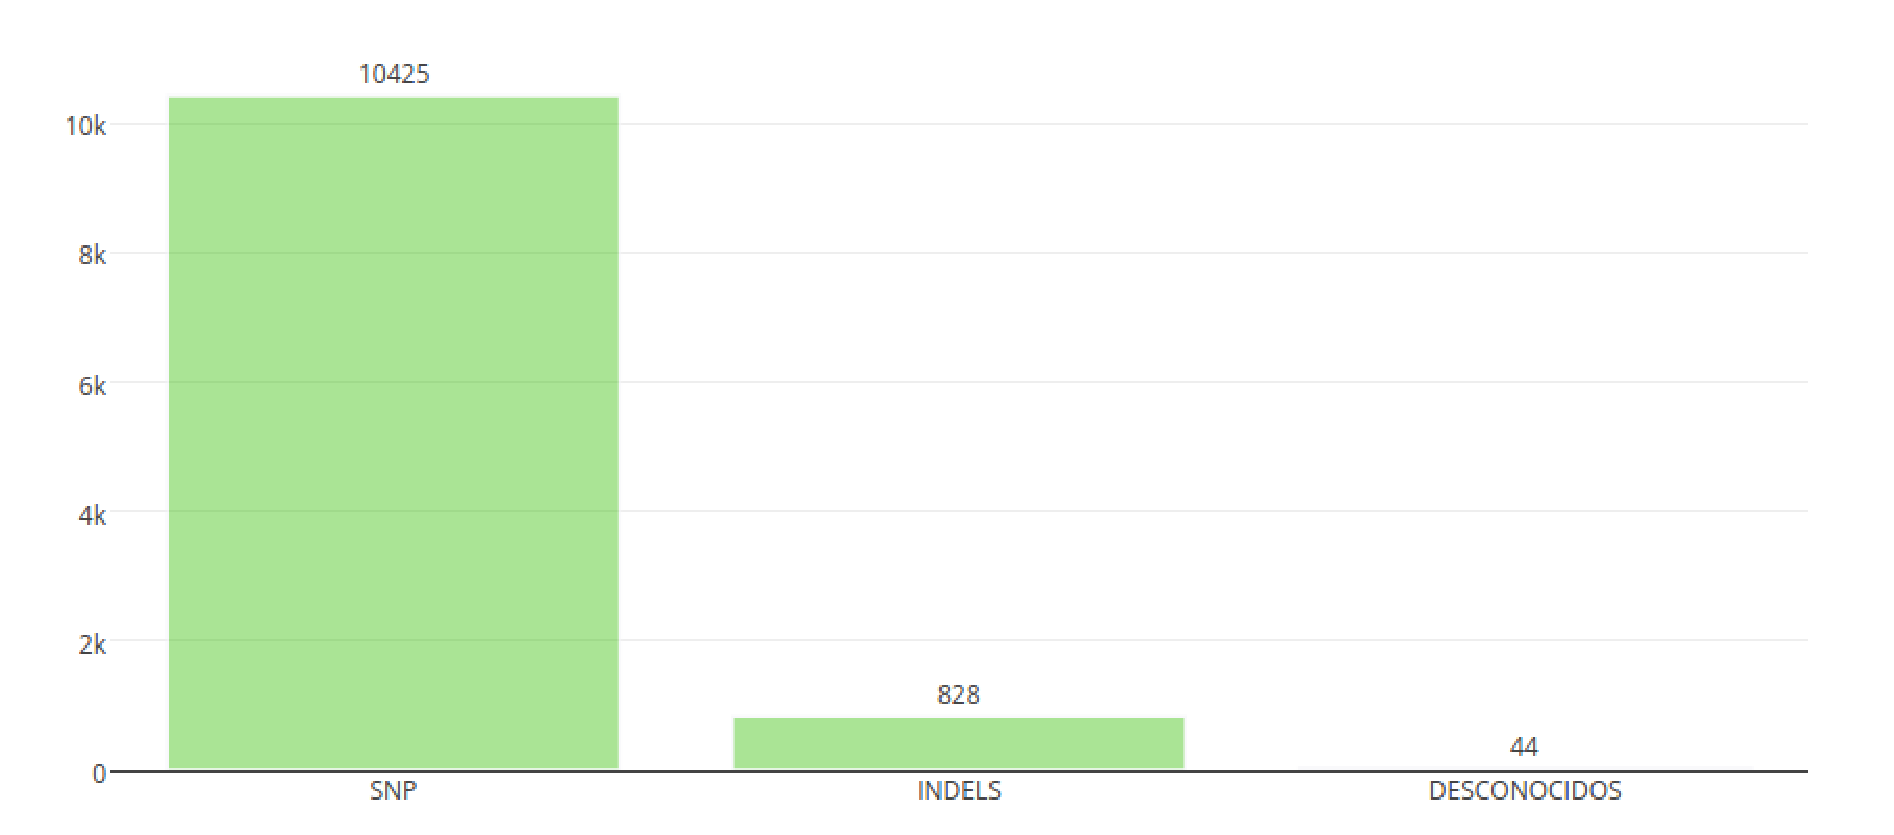
\includegraphics[width=0.5\textwidth]{Kap2/variantescalibradas}}
	\subfigure[Variantes calibradas]{
		\label{f:calibradas}
		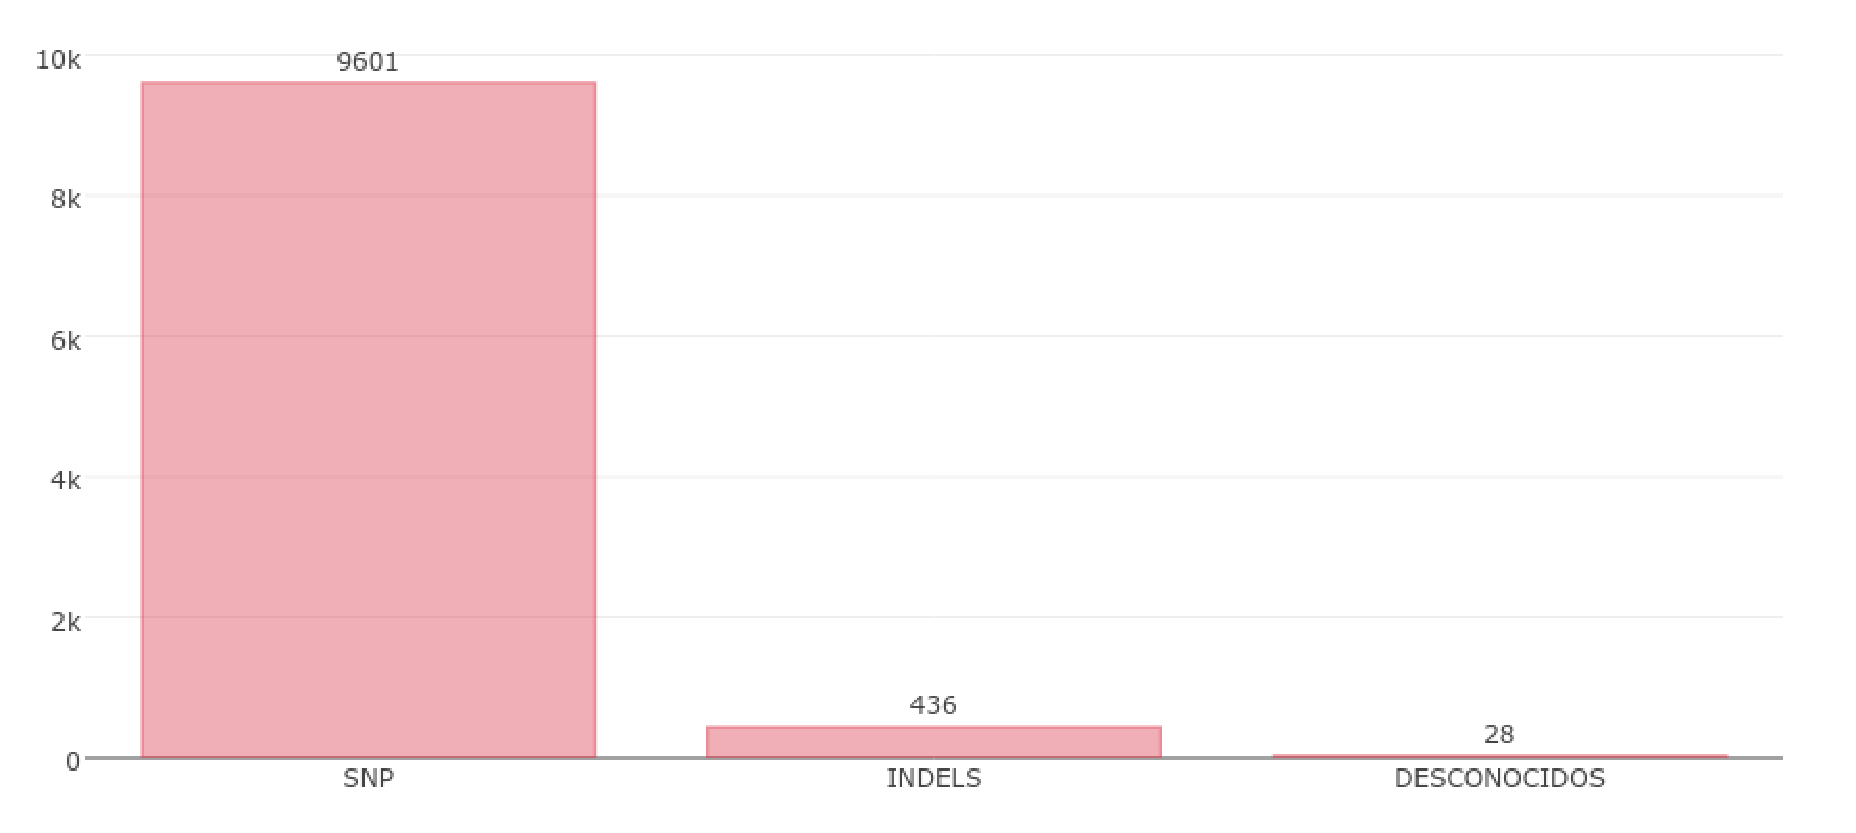
\includegraphics[width=0.5\textwidth]{Kap2/variantesillumina}}
	\caption{Variaciones de la muestra}
	\label{f:histogramas}
\end{figure}

Se realizo un distribución de las variantes según cada técnica sin filtrado (para el caso de omics) para el siguiente gráfico mostrados en las siguientes figuras  \ref{fig:tabla1} y \ref{fig:distribucion} :

\begin{figure}[H]
	\centering
	\includegraphics[width=0.4\textwidth]{Kap2/latex_table}
	\caption{Distribución de variantes a lo largo de los cromosomas} \label{fig:tabla1}
\end{figure}

\begin{figure}[H]
	\centering
	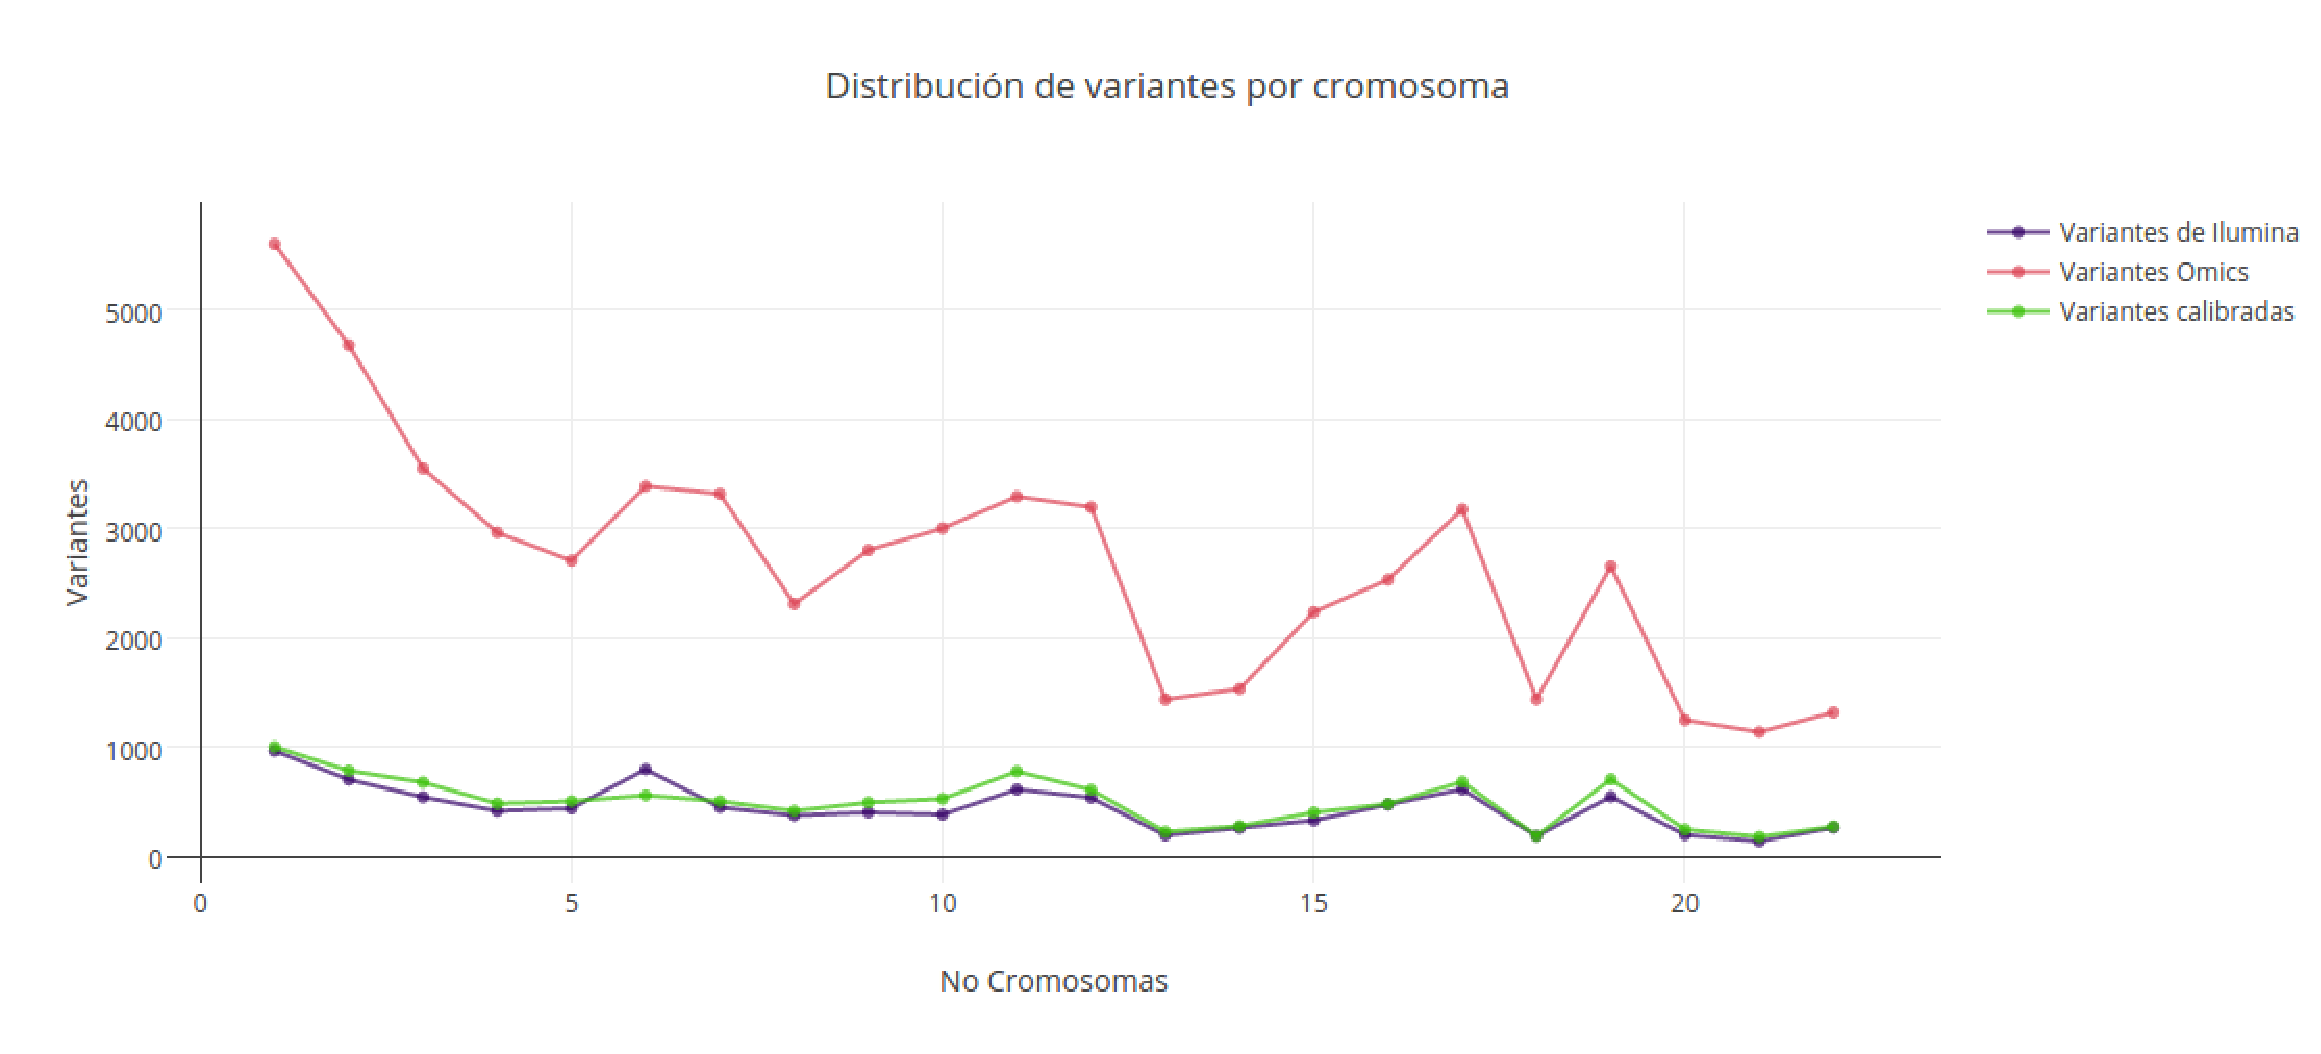
\includegraphics[width=1\textwidth]{Kap2/variaciones}
	\caption{Distribución de variantes a lo largo de los cromosomas} \label{fig:distribucion}
\end{figure}

Se observa la distribución de las variantes a lo largo del genoma, inicialmente las variantes obtenidas son en grandes cantidades para el modulo de omics, pero conservan el patrón de distribución es similar para los tres casos,incluso cundo se realiza el hard filterin las diferencias en cuanto a la distribución de las variaciones es similar, siendo la mayor para el cromosoma 1 y la menor para el cromosoma Y. \\

Al realizar la comparación entre los dos archivos vcf se obtuvieron los siguientes resultados los archivos vcf de Illumina y los de Omics comparten 49.4 \% d y 44.0 \% de las variantes, y difieren entre un 50.6\% para Illumina y 56-0\% para los datos de omics pipe. Como se refleja en el siguiente diagrama (\ref{fig:diagrama}):

\begin{figure}[H]
	\centering
	\includegraphics[width=0.3\textwidth]{Kap2/diagrama1}
	\caption{Diagrama de relación entre variantes comunes de Omics y de Illumina} \label{fig:diagrama}
\end{figure}

\subsection*{Variantes de exoma vs variantes de omics}

Una vez obtenidas las regiones se realizo el proceso de hard filtering para el vcf obtenido por el pipe de omics y por el generado por vcftools teniendo los siguientes resultados mostrados por la tabla \ref{tabla:tabla2}: \\

\begin{table}[H]
	\centering  
	\begin{tabular}{|l|l|l|l|l|}
		\hline
		& \multicolumn{4}{c|}{\textbf{Variantes Exoma}} \\
		\cline{2-5} 
		& SNP  & Indels & Desconocida & Total \\ \cline{2-5}
		\hline 
		\multirow{1}{4cm}{Variantes Omics} & 30893 & 3324 & 0 & 34217 \\ \cline{2-5}
		\hline 
		\multirow{1}{4cm}{Variantes Públicas} & 29749 & 3101 & 0 & 32850 \\ \cline{2-5}
		\hline
	\end{tabular}
	\caption{Tabla de Variantes obtenidas a partir de un exoma.}
	\label{tabla:tabla2}
\end{table} 

Donde se observa una diferencia de 1367 en el total de las variantes encontradas, para los SNPs se encuentra una diferencia de 1144 y 223 para los indels, no se encuentran variantes que no hayan sido correctamente identificadas. Presentado en los siguientes gráficos \ref{f:histogramas2} \\

La distribución de las variantes a lo largo de los cromosomas se presenta en la siguiente tabla \ref{fig:tabla2}:

\begin{figure}[H]
	\centering
	\includegraphics[width=0.4\textwidth]{Kap2/latex_table2}
	\caption{Distribución de variantes a lo largo de los cromosomas para los exomas.} \label{fig:tabla2}
\end{figure}

\begin{figure}[H]
	\centering
	\subfigure[Variantes obtenidas por Omics]{
		\label{f:variantesexo1}
		\includegraphics[width=0.3\textwidth]{Kap2/variantesexo1}}
	\subfigure[Variantes públicas]{
		\label{f:variantesexo2}
		\includegraphics[width=0.25\textwidth]{Kap2/variantesexo2}}
	\caption{Variaciones de la muestras dentro del exoma}
	\label{f:histogramas2}
\end{figure}

Y la representación gráfica de las variantes sobre la distribución a lo largo de los cromosomas figura \ref{fig:variaciones2}:

\begin{figure}[H]
	\centering
	\includegraphics[width=1\textwidth]{Kap2/variaciones2}
	\caption{Distribución de variantes a lo largo de los cromosomas para los exomas} \label{fig:variaciones2}
\end{figure}

En la figura \ref{fig:variaciones2} se observa el comportamiento de la distribución de las variantes para los datos públicos y los datos obtenidos para el pipeline donde se encuentran un comportamiento similar de la distribución, pero se observa que aún hay una mayor cantidad de variantes obtenidas por el pipeline. En la siguiente figura se observa el comportamiento de las variantes públicas con respecto a las variantes del pipeline. 

\begin{figure}[H]
	\centering
	\includegraphics[width=0.3\textwidth]{Kap2/diagrama2}
	\caption{Diagrama de relación entre las variantes publicas y las obtenidas por el pipeline} \label{fig:diagrama2}
\end{figure}

El diagrama de la figura \ref{fig:diagrama2} muestra la comparación de las variantes obtenidas y su respectiva concordancia done el 100\% del exoma esta representado en las variaciones encontradas mienteras que un 96\% de las variaciones obtenidas por omicspipe son un 96\% dejando solo un 4\% de las variantes no encontradas dentro del exoma publico. \\

GATK realiza un reporte de la evaluación cunado se comparan dos archivos de distintas variaciones, este puede ser abierto como un archivo de texto o cargado directamente en R utilizando la librería \textit{gsalib} quien lee el archivo \textit{merged.eval.gatkreport}, esto genera una lista que tiene anidados varios data.frame, dentro de ellos para este caso se tomo el \textit{ValidationReport)} que genera una tabla con los falsos positivos, falsos negativos, calcula la sensibilidad y la especificidad  y el valor predictivo positivo (PPV). Que para nuestro caso de nuestro exoma se encuentran en la tabla \ref{tabla:tabla3}:

\begin{table}[H]
	\begin{center}
		\begin{tabular}{|l|l|l|l|}
			\hline 
			\textbf{TP} & \textbf{FP} & \textbf{FN} & \text{TN} \\
			\hline 
			32110 & 0 & 1033 & 0 \\ \hline
		\end{tabular}
		\caption{Tabla de validación 1.}
		\label{tabla:tabla3}
	\end{center}
\end{table}

La tabla \ref{tabla:tabla3} refleja que para el conjunto de datos no hay falsos positivos ni verdaderos negativos, pero si falsos negativos, es decir 1033 variantes del conjunto de datos obtenidos. (\textit{GATK para calcular estas métricas compara contra una base de datos que el usuario disponga para determinar variantes existentes}).  La tabla \ref{tabla:tabla4} muestra la sensibilidad, especificidad y el valor predictivo positivo (PPV).

\begin{table}[H]
	\begin{center}
		\begin{tabular}{|l|l|l|}
			\hline 
			\textbf{Sensibilidad} & \textbf{Especificidad} & \textbf{PPV} \\
			\hline 
			96.88 & 100 & 100 \\ \hline
		\end{tabular}
		\caption{Tabla de validación 2.}
		\label{tabla:tabla4}
	\end{center}
\end{table}

Donde se tiene que existe una sensibilidad de 96.88\%, una especificidad del 100\% y un PPV de 100.Además después de la limpieza de los datos se realizo la anotación del archivo vcf obtenido, para el gen CYP2C19 utilizando la versión gráfica de annovar \cite{Yang2015} y obteniéndose el siguiente resultado: \\

\texttt{chr10,96541616,96541616,G,A,exonic,CYP2C19,synonymous SNV, CYP2C19:}

\texttt{NM\_000769:exon5:c.G681A:p.P227P} \\

La representación escrita informa el cromosoma, la posición dentro del genoma y el cambio de posición en el genoma, las siguiente es el cambio Guanina por Citocina (representado por sus letras) tipo de variación que en este caso es sinónima, el nombre del gen, su identificador, vubicación exonica y cambio en la posición del exón, finalmente se tiene el cambio en la proteína (No sigue exactamente la nomenclatura de HGVS), esta variación se confirmo también realizando la visualización por medio de la herramienta IGV conectado al clúster.

\begin{figure}[H]
	\centering
	\includegraphics[width=0.9\textwidth]{Kap2/IGV}
	\caption{Imagen de la variante presente en el exoma público} \label{fig:igv}
\end{figure}

\section{Discusión}

\subsection*{Preprocesamiento}

La revisión de las metricas dadas por el FASTQC report muestran el estado de como están las secuencias antes de ser procesadas, aunque a nivel experimental no dependiendo de las condiciones y el tipo de muestra los niveles de calidad terminan bajando de manera sustancial y depende del analista tomar la decisión de remover secuencias o mantenerlas ya que los diferentes módulos presentan diversas meticas de evaluación de las secuencias \cite{Babraham2016}. \\

El presente conjunto de secuencias FASTQ se encuentra con buenos parámetros de calidad, aunque algunos módulos presentan falla, el percentil, el porcentaje de GC, la distribución del largo de las secuencias, los niveles de duplicación de las secuencias y los valores de K-mer y las secuencias en secuencias cortas de 7 nucleótidos, representan que dentro del conjunto de datos estas secuencias cortas están en la parte inicial de la mayoria de las lecturas obtenidas en la muestra y que posiblemente son secuencias duplicadas que no pertenecen al conjunto de secuencias real, a pesar de que no se encuentran adaptadores, ni representaciones al final de las lecturas. Esto puede llevar a dos caminos, el primero que estas secuencias sean parte de un adaptador (llama la atención que no se encuentren al final de la secuencia)  o que sean errores propios del proceso de secuenciación durante la hibridación de las secuencias y sean representados como duplicaciones de las secuencias originales \cite{Babraham2016}\cite{Pirooznia2014}. \\ 

Además existen otras características que pueden generar impactos negativos dentro del analisis de datos de NGS divididas en dos grupos \cite{Zhou2013}: 

\begin{enumerate}
	\item Lecturas con baja calidad: Las calidades de las lecturas generadas por un secuenciador pueden degradarse durante el proceso de corrido y es común ver fallas al final de la lectura o tener secuencias duplicadas a partir de la amplificación por PCR durante la construcción de las librerías \cite{Zhou2013}.
	\item Contaminación de las lecturas de especies conocidas o no conocidas en la secuencia objetivo, este error es frecuente y puede se causado por un experimento artificial durante la preparación de la muestra, la construcción de la libreria o otro paso experimental, sin embargo las muestras de ADN pueden contener algunos nucleótidos de otras especies, las cuales son difíciles de excluir de manera experimenta y por lo tanto si se cree que hay una contaminación lo ideal es realizar un triming de las secuencias para remover la contaminación. \textbf{Nota:} Siempre y cuando estén en una baja proporción \cite{Zhou2013}.
\end{enumerate}

Las secuencias que se  observan pueden ser duplicados de PCR que son un problema critico cuando los fragmentos están sobre amplificados durante la preparación de las librerías, estos duplicados pueden aumentar a frecuencia alelica e incluir una detección erronea de variantes, esto es muy común los datos de metagenomica, pero en nuestro caso los datos no son datos de metaegenomica si no de un solo individuo llama la atención de que solo esten al inicio de las lecturas y que el final de las lecturas este adecuado esto podría indicar que más que un duplicado de PCR pueda ser un error de secuenciación al inicio de cada nuevo ciclo.\cite{Pandey2016}. \\

Teniendo en cuenta lo anterior se puede inferir que las secuencias duplicadas son bajas y que la calidad de los datos obtenidos son adecuados para continuar con el procesamiento de las secuencias FASTQ, dentro del pipeline se cuenta con una herramienta para remover las secuencias duplicadas (PICARD) y así obtener una calidad optima de los datos.

\subsection*{Variantes obtenidas}
\subsubsection*{Variantes de illumina y omics pipeline}

En los datos obtenidos para illumina inicialmente reflejados en la tabla \ref{tabla:final}, muestran una alta discordancia ya que inicialmente las variantes no se les aplicó un segundo filtro, siguiendo las recomendaciones de  GATK , donde por el pipeline de Omics tiene por defecto el variant quality score racalibration (VQRS) que se basa en machine learning para filtrar las variantes y generar una alta sensibilidad verdadera, que es el método más recomendado, pero tiene limitaciones estadísticas y es más robusto que el hard filtering, este es recomendado para datos pequeños \cite{Auwera2014}. \\

Al realizar una calibración de los datos con la calidad y con hard filtering en GATK se obtiene una similitud entre la cantidad de variantes obtenidas por omics con respecto a Illumina, pero aún es posible ver que la distribución de las variantes es similar para ambos conjuntos de datos (véase la figura \ref{fig:distribucion}) y se acerca más después de realizar el filtrado. Esto se presenta debido a que no existe una formula para determinar cuales anotaciones y filtros son adecuados, además el VQSR genera datos de entrenamiento para determinar las variaciones y se hacen recomendaciones según lo que se ha observado empíricamente dentro del desarrollo de los algoritmos \cite{Auwera2014}. \\

A pesar de que la distribución de las variante es similar, aun con el filtrado de las variantes existe que la concordancia entre ambas técnicas tiende a ser del 50\% (véase la figura \ref{fig:diagrama}), aunque illumina utiliza GATK la versión implementada es la 1.6 que en este momento no cuenta con documentación (https://www.broadinstitute.org/gatk/guide/version-history) que illumina utiliza la versión 1.6 y la función UnifiedGenotyper que presenta algunas inconsistencias para la identificación de indels, mientras que la versión de GATK 3.5 utiliza la función HaplotyperCaller que mejora el llamado de variantes, y corrige algunas inconsistencias para la identificación de indels \cite{ORawe2013}. Además es la función recomendada para organismos diploides, este se enfoca en dos tipos de identificación inicialmente los SNPs y los indels, y puede identificar cuando hay varios tipos de variantes cercanas a otras \cite{Auwera2014}. \\

Illumina no provee los parametros utilizados para hacer el llamado de variantes lo que dificulta la comparación entre este pipeline y las variantes reportadas por illumina, además el formato del VCF es el 4.1 y en la mayoria de las variantes no reporta el valor de la Qual (calidad) para hacer un filtro con el archivo aunque para GATK los valores para el llamado de variantes no son modificados de manera significativa si se realiza un filtro de este tipo \cite{Hwang2015}. Además de que la combinación de BWA con HaplotypeCaller, presentan una mejora con respeto a la identificación de SNPs (BWA-men) y HaplotypeCaller para la identificación de indels \cite{Cornish2015}.

\subsubsection*{Variantes con un exoma NA12878.}

Para este estudio se utilizo una muestra del genoma completo de la muestra NA12878 son de 34,886 variaciones \cite{Cornish2015} en el presente estudio 32850 y el pipeline obtuvo un total de 34217, lo que permite inferir que las variante identificadas son solo de 2036 variaciones (dependiendo de las muestras y los genes que fueron secuenciados) y que se realizo un muestreo partir de un archivo bed. Además si se aplica un filtro para retirar las variaciones con baja calidad, el llamado de variantes de GATK mejora de manera significativa si necesidad de hacer cambios en el preprocesamiento de los datos \cite{Warden2014} \\

Las dos resultados presentan una distribución similar en cuanto a las variantes por cromosoma y no hay variantes desconocidas dentro de la muestra,esto se debe a la alta curación que tiene este exoma, la figura \ref{fig:variaciones2} presenta la distribución a lo largo de los cromosomas donde se presenta leves diferencias entre los datos públicos y los datos generados por el pipeline con una diferencia del 4\% entre las dos resultados, no existen falsos positivos ni verdaderos negativos identificados dentro del conjunto de los datos del pipeline, se presenta una sensibilidad del 96\% que es alta , dado que las calibraciones y los algoritmos presentan falencias reales para la identificación de variantes \cite{Auwera2014}. Esto se puede corregir por dos vias, aplicando un filtro de Quality by Depth (QD) >= 4 and Fisher Strand Bias (FS) =< 30 para dar un balance  a la sencibilidad y la especificidad \cite{Tsai2016} o aplicando múltiples pipelines.\\

La no existencia de falsos negativos y verdaderos positivos, esta supeditada al hecho de que se tomo una muestra de las muestras comunes, es decir que tanto en la muestra a comparar con la obtenida se van a ver las posiciones entre los datos analizados, aún con esta limitante acerca de la posición de las variantes en la región génomica se logra ver el error que se esta obteniendo dentro del pipeline, aunque la precisión es alta y no hay false descovery rate (FDR).\\

La sensibilidad de un solo pipeline esta en promedio de 95\% al 99\% ,que esta dentro del rango de aceptabilidad para la identificación de las variantes \cite{Liu2013}. Para nuestro pipeline tenemos una precisión de 100\%. Lo que muestra que hay baja probabilidad de error.\\

Al realizar la anotación se logro encontrar una de las variantes reportadas para el exoma, en el gen CYP2C19 en la misma posición reportada, con la misma variación mostrando la concordancia entre los resultados del pipeline y la muestra original. \\

Para ambos estudios se presentan archivos intermedios de gran tamaño como son los bam y bai que permiten la visualización de las variantes que pesan entre 6 y 15 gigas para un exoma completo, los datos iniciales pueden pesar entre 1 y 3 gigas (fastq) dependiendo de la cantidad de genes que se hallan secuenciado, lo que requiere de la disponibilidad de un computo para su almacenamiento y procesamiento. 

\section{Conclusiones}

La validación de un pipeline para la identificación de variantes requiere la utilización de herramientas computacionales de HPC para hacerse de manera eficiente. Es necesario que se tengan conocimientos de programación básica y biología molecular, con el fin de definir los parámetros óptimos para la implementación un pipeline.\\ 

La cantidad de herramientas y parámetros para aplicar son diversos y dependen del investigador decidir cuales son los mejores y que filtros van a ser utilizados, dado que a pesar de la existencia de protocolos no hay un consenso de cual o cuales son los mejores y estos dependen del conjunto de datos obtenido. \\ 

El llamado de variantes es bueno para el presente estudio, pero hay la posibilidad de mejorar la implementación de los parámetros de filtrado y el proceso de anotación (implicación del cambio de las variantes), además generar un pipeline alternativo para la verificación de las variantes que están siendo identificadas y poder aumentar la sensibilidad. \\

Es necesario crear o generar la manera de optimizar los tiempos de ejecución de las tareas, de una manera más eficiente a la dada por el omics pipe.

\section*{Resumen}

Se realizo la implementación y validación de un pipeline para la identificación variantes a partir de secuencias de exomicas a partir de muestras de pacientes colombianos y del genoma público de la muestra NA12878 donde se identificaron las variantes que presentes en el mismo, teniendo en cuenta las buenas practicas para el análisis de variantes lo que permitió desarrollar un mecanismo para obtener variantes de buena calidad.
\chapter{Modelo de integración de datos}

El mayor de los retos aplicado al análisis de variantes, es desarrollar herramientas que permitan al investigador acceder a la información fácilmente y que pueda tener una base de datos,donde pueda consultar, analizar y actualizar la información de sus experimentos \cite{Li2014}.En el campo clínico esto representa un reto aun mayor dado que se hace necesario recolectar los datos genéticos junto con los datos clínicos para poder hacer análisis más acertados y a gran escala \cite{Paila2013}.\\


Este capítulo presenta el desarrollo de un sistema de información para la gestión de información clínica y genómica, desde el diseño e implementación de la base de datos.Este capítulo esta   organizado en 3.1. Diseño e implementación de datos. 3.2. Gestión de datos clínicos y genómicos. 3.3. Conclusiones y  Resumen.

\section{Diseño e implementación del modelo de datos}

\subsubsection{Datos}

Se tomaron una  250 pacientes previa autorización  del laboratorio Genetix S.A.S de los cuales solo 228 contaban con consentimiento informado para utilizar la información con fines de investigación.  La información disponible, se cargo en un archivo de texto plano con la siguiente información: Edad,genero y diagnóstico y adicionalmente para cada paciente se tenían las variantes en un archivo csv, resultado de la anotación realizada en con wAnnorvar según el pipeline implementado en el capítulo 2.\\

A continuación proponemos la utilización de una base de datos con información clínica  y las variantes obtenidas a partir del pipeline. La figura \ref{fig:flujo2} representa el esquema de datos que fue utilizado para realizar la integración de la información dentro de la base de datos. \\ 

\begin{figure}[h!] 
	\centering
	\includegraphics[width=0.5\textwidth]{Kap3/flujo2}
	\caption{Esquema de datos integrados} 
	\label{fig:flujo2}
\end{figure}

Teniendo en cuenta la información a utilizar se diseño el esquema EER  que muestra la figura \ref{fig:t} con las tablas generadas por la aplicación para crear la base de datos propias de Django y las tablas de para la gestión del las variantes junto con la historia clínica.

\begin{figure}[H]
	\centering
	\includegraphics[width=0.9\textwidth]{Kap3/modeloEER}
	\caption{Modelo entidad relación} \label{fig:t}
\end{figure}

Las tablas diseñadas para gestionar las variantes y las historias clínicas son gene\_variants\_paciente que contienen:

\begin{itemize}
	\item Edad: 0-99. Los recién nacidos  o menores de un año tienen una edad de 0.
	\item Sexo: F o M según corresponda.
	\item Descripción: Que corresponde a la información clínica disponible.
\end{itemize} 


Las variantes con su historia clínica fueron cargadas mediante un script en bash disponible en https://github.com/jevelezse/variantesBD/blob/master/carga.bash, donde se toman los archivos .csv de annovar junto con los archivos de texto que tienen la información clínica del paciente distribuida de la siguiente forma:

\section{Gestión de datos genómicos y clínicos}

Los resultados obtenidos fueron una aplicación con una interfaz que permite a los usuarios con poco conocimiento de  programación  analizar los datos de variantes y su resumen de la historia clínica. \\

\begin{figure}[h] 
	\centering
	\includegraphics[width=0.4\textwidth]{Kap3/admin_django}
	\caption{Interfaz de ingreso para  administrar la base de datos.} \label{fig:admin}
\end{figure}

Inicialmente la figura\ref{fig:admin}, muestra la solicitud de usuario y contraseña para acceder a la aplicación, es diferente a la base de MySQL, pero  puede tener  una contraseña igual o diferente a la de la base de datos.

\begin{figure}[h] 
	\centering
	\includegraphics[width=0.5\textwidth]{Kap3/django_admin}
	\caption{Interfaz de administración.} \label{fig:admin2}
\end{figure}

La figura \ref{fig:admin2}, muestra el sitio de administración donde se encuentran los usuarios permitidos, las bases de datos a consultar y muestra un histórico de las actividades recientes. \\

Desde esta interfaz se puede agregar un grupo, más usuarios, pacientes y/o variantes dando click en el signo más sin necesidad de hacer la carga directa a MySQL ya que Django se encarga de hacer la carga, lo que permite actualizar los cambios que se reporten para la variante, por ejemplo variantes que por su alta frecuencia poblacional dejan de ser variantes y se convierten en referencias. \\

\begin{figure}[h] 
	\centering
	\includegraphics[width=0.5\textwidth]{Kap3/ingresar_paciente}
	\caption{Ingreso de pacientes.} \label{fig:pacientes}
\end{figure}

En la figura \ref{fig:pacientes} se muestra el formulario para ingresar una nueva historia o de modificar una historia clínica de un paciente de manera manual.

\begin{figure}[h] 
	\centering
	\includegraphics[width=0.5\textwidth]{Kap3/consulta}
	\caption{Consulta a variantes} \label{fig:consulta}
\end{figure}


La figura \ref{fig:consulta} muestra una consulta de las variantes que se tienen cargadas en la base de datos para el gen BRCA1, donde nos muestra una consulta de las variantes con su anotación  filtrada mediante un script de python antes de cargar las anotaciones de la tabla obtenida por annovar para cada paciente. Desde esta misma interfaz se puede hacer consultas de pacientes que se deben eliminar, en la parte inferior se encuentra la opción.\\

Si se desea hacer modificaciones a los datos del paciente también es posible hacerlo desde esta misma interfaz seleccionando el código del paciente, que lleva a la tabla de genes\_varante\_paciente que contiene el formulario de la historia clínica con los datos cargados para ser modificados. 

La importancia de gestión aplicada al manejo de datos clínicos y de información genética es de vital importancia dado que existen miles de anotaciones que requieren de scripts para cargarlos las anotaciones y como es este caso el historial clínico del paciente \cite{Paila2013}. \\

La aplicación desarrollada para crear y gestionar una base de datos aplicada una bioinformática con aplicaciones a la medicina, es necesario que la base de datos provea las consultas para soportar las decisiones sobre un paciente en especifico teniendo en cuenta sus datos,la relación con datos de otros pacientes y los datos de exomas, además de los datos relacionados con los familiares en caso de que se encuentren estos datos. Mostrando que es posible realizar una integración adecuada de los datos bioinformáticos y clínicos utilizando bases de datos relacionales, con una buena respuesta en las consultas. \cite{Sujansky2001}.

Los datos fueron consultados  desde mysql y cargada a librería de python pandas \cite{mckinneypandas}.

\section{Conclusión}

La utilización de aplicaciones en Django permite que un bioinformático diseñe e implementar bases de datos aplicadas al diagnostico clínico, donde se puede guardar y gestionar toda la información obtenida de un paciente, lo que permite hacer análisis a profesionales Médicos y biólogos fácilmente. Una vez ha sido implementa la base de datos también es posible aplicar técnicas de minería de datos para optimizar los análisis de la información. \\

\section*{Resumen}

En este capitulo se presento el proceso de diseñar e implementar un sistema de información para la gestión de datos clínicos y genómicos, dada la importancia de tener toda la información integrada para hacer futuros análisis. Se utilizo la herramienta de Django como gestor de la base de datos,se transcribió las información clínica y se cargaron las variantes obtenidas para cada paciente, como resultado se genero un sistema de información que permite realizar consultas de variantes con las características clínicas de los pacientes.   
\chapter{Modelo de minería de datos}

La necesidad de comprender los procesos biológicos que están implicados en las distintas enfermedades, a partir de la gran cantidad de datos biológicos que hay disponibles como las secuencias genómicas, los microarreglos, las interacciones proteicas, las imágenes biomédicas entre otros. Además la rápida adopción de las historias clínicas electrónicas proporciona una oportunidad de realizar investigaciones a gran escala. Por lo tanto las técnicas de minería de datos para el descubrimiento de conocimiento a partir de la obtención de información proveniente de diferentes fuentes son cada vez mas importantes en la investigación biológica y médica \cite{Wang2017}.\\

El mayor reto de la minería de datos genómicos esta en la extracción de información relevante de grandes volúmenes de datos clínicos y transformarlos en conocimiento, los mayores retos están en: a) La recolección de los datos clínicos y genómicos, b) recuperación de información relevante de datos y c) extracción de nuevos conocimientos de la información \cite{Farid2016}. \\  

Este capitulo esta organizado en análisis exploratorio de los datos que se describe en la sección 5.1, el siguiente, es el analisis textual de información clínica que es discutido en la sección 5.2 en este apartado se describe el analisis de asociación de variantes con la información clínica. Finalmente, el apartado de 5.3 se presentan las conclusiones junto con el resumen del capitulo. 

\section{Análisis exploratorio de los datos}

Se realizo el análisis exploratorio de la información contenida dentro de la base de datos.Se tomo una muestra de 250 pacientes donados por el laboratorio Genetix S.A.S de los cuales solo 228 contaban con consentimiento informado para utilizar la información con fines de investigación.\\

\begin{figure}[h!]
	\centering
	\includegraphics[width=0.5\textwidth]{Kap4/general}
	\caption{Distribución de rango de edades y géneros de los pacientes}
	\label{fig:general}
\end{figure}

\begin{figure}[H]
	\centering
	\subfigure[Distribución de variantes según su tipo.]{
		\label{f:generosgeneral}
		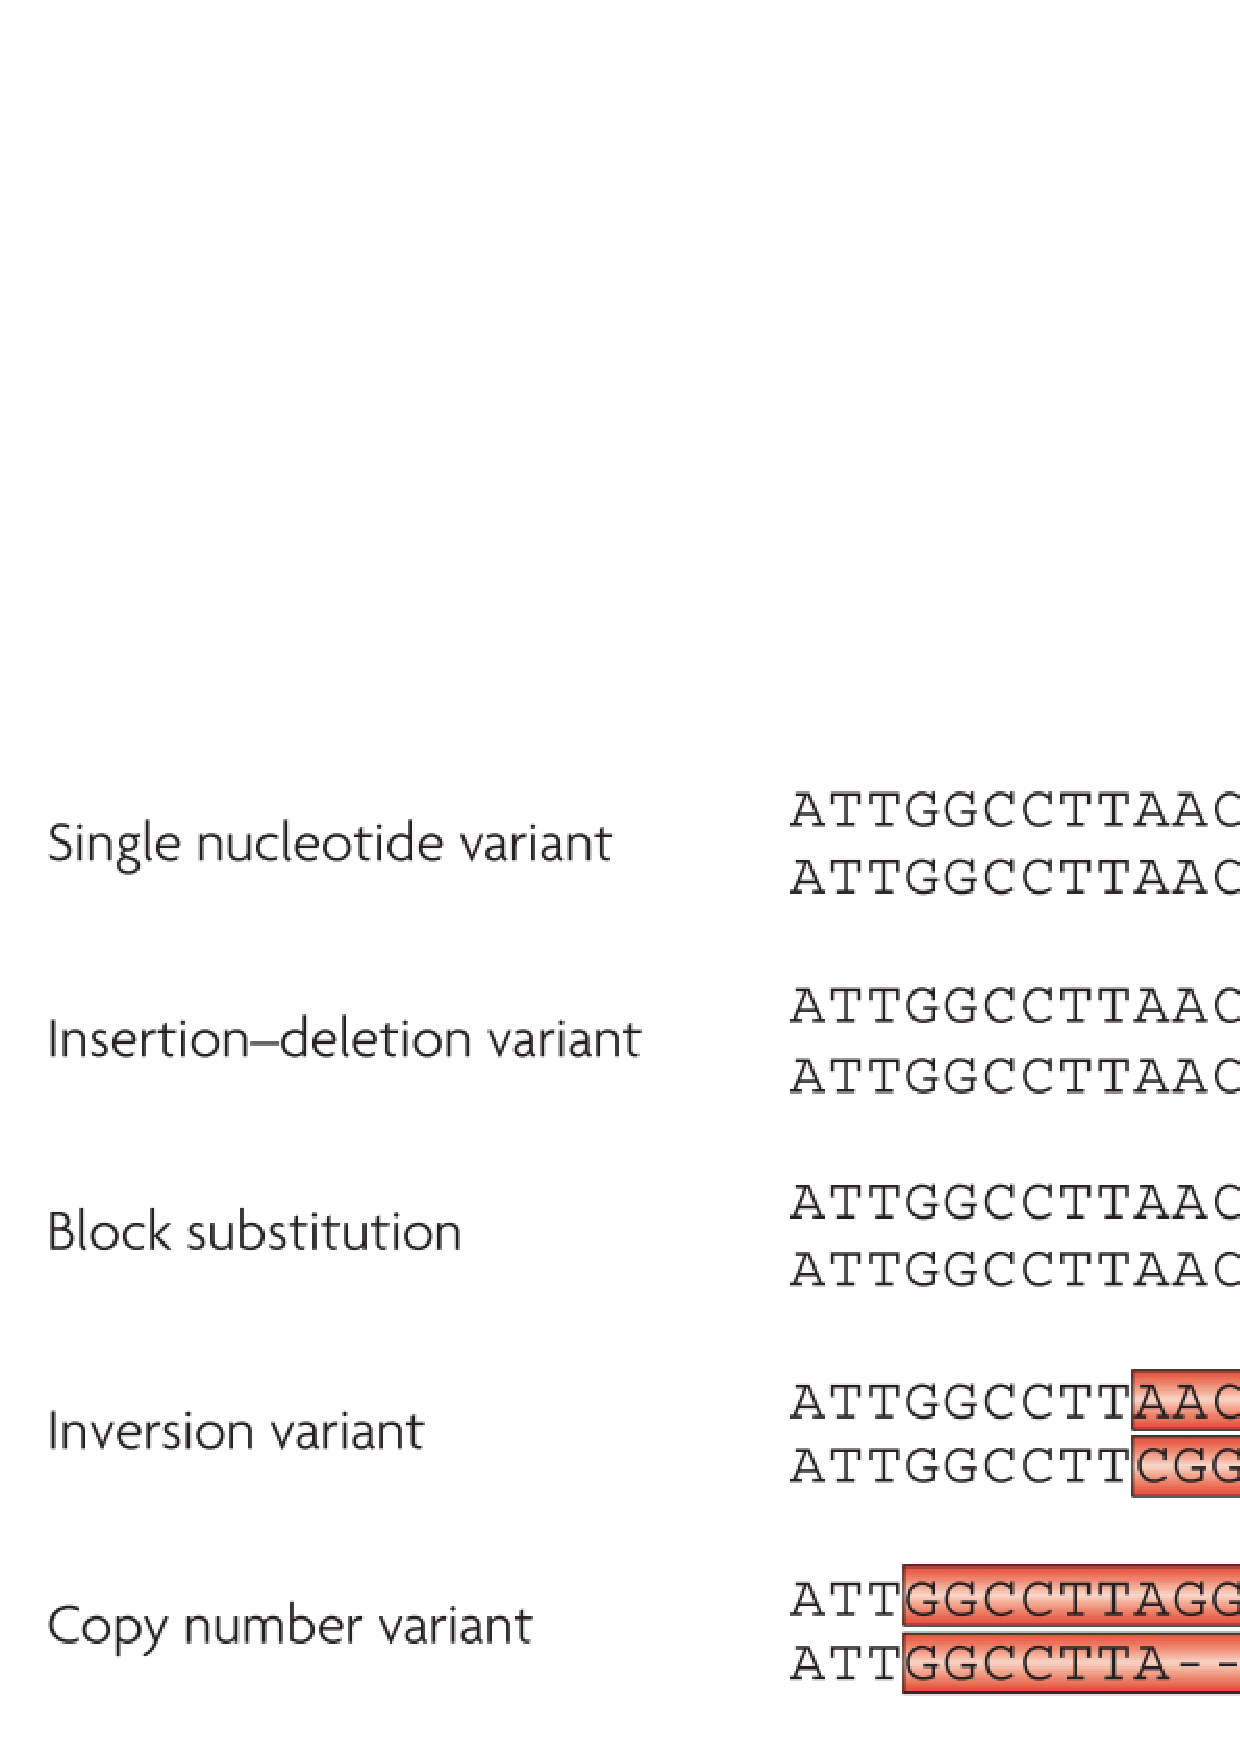
\includegraphics[width=0.35\textwidth]{Kap4/variantes.png}}
	\subfigure[Distribución de variantes por rango de edad]{
		\label{f:variantedad}
		\includegraphics[width=0.55\textwidth]{Kap4/edad.png}}
	\caption{Distribución del tipo de variantes}
	\label{f:variantesgeneral}
\end{figure}

La base de datos contiene 228 pacientes de los cuales 133 son de género femenino y tienen un total de 468.485 variantes y 95 de género masculino con 345.239 de variantes obteniendo  un total de 803.878 variantes. La  figura \ref{fig:general} representa la distribución de pacientes por rango de edades y la figura \ref{f:variantesgeneral} representa la distribución de variantes según su tipo. En la figura \ref{f:generosgeneral} muestra el número de variantes que son sinónimas y no sinónimas siendo las más frecuentes en la población, a  nivel mundial se conoce que estos son lo tipos de variantes más frecuentes\cite{Fu2013}.\\

Las variantes desconocidas son el tercer tipo de variante más frecuente dado que aún existe el problema de selección del transcripto para realizar la nomenclatura adecuada de las variantes, por lo que el anotador informa que son desconocidas \cite{McCarthy2014}. La figura\ref{f:variantedad} muestra la distribución de las variantes identificadas según el rango de edad, siendo el rango con mayor número de variantes los pacientes que se encuentran entre las edades de 0 a 10 años, dado a que es la población más representada dentro de la base de datos. \\

El estado alélico de las variantes (cigocidad) que se encuentran dentro de la base de datos se dividen en heterocigotas 458639 que corresponden al 57,05\% del total de las variantes  y homocigotas 345239 que corresponden al 42,95\%. La distribución de la cigocidad de las variantes se puede explicar desde el error que se puede generar en la identificación de las variantes dado que durante el llamado  de variantes es posible que una variante homocigota se catalogue como heterocigota o si durante el proceso de secuenciación se identifican erróneamente los nucleótidos \cite{Babraham2016}\cite{Pirooznia2014}. 


\section{Análisis textual de información clínica.}

 
\subsection{Preprocesamiento.}

El proceso de limpieza y nacionalización de texto se realizo de la siguiente manera:

 \begin{enumerate}
 	\item Remoción de stop words en español, tildes y caracteres especiales como  la letra ñ y todos los documentos se unificaron en letras minúsculas.
 	\item Teniendo en cuenta la información clínica se creo un diccionario de sinónimos, donde se reemplazaron palabras que hacen referencia a una misma característica.
 	\item Calculo de la frecuencias de palabras dentro de los documentos. 
 	\item Se removieron las palabras pam,pacientes, secuenciación y gen dado que no son un factor diferenciador de los documentos.  	  
 \end{enumerate}

\subsection*{Resultados}

Los resultados que se obtuvieron para la frecuencia de palabras fueron seno, cáncer, síndrome, sospecha y años. La figura \ref{fig:sin} muestra las primeras 30 palabras más frecuentes y la nube de palabras de todos los documentos.\\

\begin{figure}[]
	\centering
	\subfigure[Nube de palabras]{\includegraphics[width=60mm]{Kap4/sin_stop}}
	\subfigure[Frecuencia de términos]{\includegraphics[width=60mm]{Kap4/frecuecias.pdf}}
	\caption{Frecuencias sin stop words y palabras sinónimas} \label{fig:sin}
\end{figure} 

Las frecuencia de palabras nos muestra las principales características de la información clínica siendo las palabras cáncer y seno los principales fenotipos, también se encuentra la palabra síndrome que puede asociarse a diferentes  enfermedades y la palabra sospecha hace referencia a diagnósticos ambiguos que pueden tener los pacientes, una de las contribuciones de la secuenciación es que basado en el fenotipo puede ayudar a un diagnóstico,entre diferentes síntomas y síndromes que pueden ser aplicados a enfermedades raras y complejas\cite{Tetreault2015a}.

\subsection{Grupos de características clínicas.}

En los procesos médicos, la relación entre los factores que pueden afectar la salud juega un papel importante. Una de las relaciones más comunes es la relación entre los genes y las enfermedades donde la secuenciación de exones tiene una alta aplicabilidad. Pero la identificación manual de este tipo de relaciones es compleja dada la cantidad de características que se pueden presentar como el diagnóstico propio de la enfermedad y/o la respuesta a los tratamientos \cite{Kawashima2017}.

La minería texto y puede ser aplicado al análisis en la medicina, donde el clustering (agrupamiento) puede ser considerado el método más importante que se utiliza en aprendizaje de maquina no supervisado que ha sido aplicado a diferentes problemas\cite{Kawashima2017}, teniendo en cuenta que no de los objetivos del agrupamiento de datos, es la  identificación de grupos naturales en datos sin etiquetas\cite{Jain2010}.

Partiendo de lo anterior el presente trabajo se implemento un modelo de agrupamiento para identificar grupos de características clínicas con la siguiente metodología:

\begin{enumerate}
	\item Cálculo de la matriz tf-idf y se normalizo. 
	\item Estimación de el número de k optimo.
	\item Implementación del algoritmo k-means.
	\item Validación de los clusters.
	\item Análisis de resultados. 	  
\end{enumerate}

\subsection{Resultados}

El cálculo de la matriz tf-idf, se realiza a partir de frecuencia invertida con la ecuación 
$${idf}_i = \log_2 \frac{|D|}{|\{d \mid t_i \in d\}|}$$
siendo $|D|$ lo que denota el número total de documentos y donde $|\{d\mid t_i \in d\}|$ en  que $t_1$ aparece, la matriz de tf-idf es calculada a partir de la multiplicación de la frecuencia de términos y la frecuencia invertida $\mathit{tf}_{i,j} \cdot \mathit{idf}_i$ \cite{Buckley1988}. 
La figura \ref{fig:IDFTF} representa la matriz IDF-TF de las palabras que se encuentran dentro de la base de datos.  

\begin{figure}[H] 
	\centering
	\includegraphics[width=0.5\textwidth]{Kap4/tfidf.pdf}
	\caption{TFIDF} 
	\label{fig:IDFTF}
\end{figure}

La selección del número optimo de K se realizo calculando el error cuadrático y el valor shiluetta  :

\begin{figure}[H] 
	\centering
	\includegraphics[width=0.5\textwidth]{Kap4/Clusters.pdf}
	\caption{Número optimo de clusters} 
	\label{fig:Clusters}
\end{figure}

\begin{figure}[H] 
	\centering
	\includegraphics[width=0.8\textwidth]{Kap4/S}
	\caption{Valor Silueta de cada cluster} 
	\label{fig:S}
\end{figure}

\begin{figure}[H]
	\centering
	\subfigure[Nube de palabras]{\includegraphics[width=80mm]{Kap4/cluster1}}
	\subfigure[Rango de edad en decadas]{\includegraphics[width=70mm]{Kap4/edadsexocluster1}}
	\caption{Cluster 1} \label{fig:c1}
\end{figure}

La figura \ref{fig:c1} representa el clúster 1 con la información clínica que presenta en (a) tenemos la frecuencia de palabras, siendo seno,síndrome y cáncer son las palabras más frecuentes, junto con ovario y familiar.

\begin{figure}[H]
	\centering
	\includegraphics[width=0.9\textwidth]{Kap4/reglasc1}
	\caption{Reglas de asociación del cluster 1} \label{fig:reglas}
\end{figure}

Las primeras 10 reglas obtenidas se representan mediante la figura \ref{fig:reglas} que muestra la asociación de dos tipos de variantes dentro del clúster 1 con el genero masculino donde se tiene que el tipo de variante es no sinónima, son pacientes de edad entre 10 y 20 años, el estado alélico de las variantes es homocigoto, para este grupo se observa una alta diferencia en las reglas ambos géneros, 


\begin{figure}[H]
	\centering
	\subfigure[Nube de palabras]{\includegraphics[width=60mm]{Kap4/cluster2}}
	\subfigure[Rango de edad en decadas]{\includegraphics[width=60mm]{Kap4/edadcluster2}}
	\subfigure[Género]{\includegraphics[width=60mm]{Kap4/Cluster2G}}
	\caption{Cluster 2} \label{fig:c2}
\end{figure}

% Please add the following required packages to your document preamble:
% \usepackage{booktabs}
% Please add the following required packages to your document preamble:
% \usepackage{booktabs}
\begin{table}[]
	\centering
	\caption{My caption}
	\label{my-label}
	\begin{tabular}{@{}|c|c|@{}}
		Rango de Edad & No. de pacientes . \\ 
		0-10          & 15                 \\
		10-20         & 9                  \\
		20-30         & 3                  \\
		30-40         & 7                  \\
		40-50         & 7                  \\
		50-60         & 2                  \\ 
		60-70         & 2                  \\
		Total         & 45                 \\
	\end{tabular}
\end{table}

donde...

\begin{figure}[H]
	\centering
	\subfigure[Nube de palabras]{\includegraphics[width=60mm]{Kap4/cluster3}}
	\subfigure[Rango de edad en decadas]{\includegraphics[width=60mm]{Kap4/edadcluster3}}
	\subfigure[Género]{\includegraphics[width=60mm]{Kap4/Cluster3G}}
	\caption{Cluster 3} \label{fig:c3}
\end{figure}

Donde ...

\begin{figure}[H]
	\centering
	\subfigure[Nube de palabras]{\includegraphics[width=60mm]{Kap4/cluster4}}
	\subfigure[Rango de edad en decadas]{\includegraphics[width=60mm]{Kap4/edadcluster4}}
	\subfigure[Género]{\includegraphics[width=60mm]{Kap4/Cluster4G}}
	\caption{Cluster 4} \label{fig:c4}
\end{figure}

Donde 

\begin{figure}[H]
	\centering
	\subfigure[Nube de palabras]{\includegraphics[width=60mm]{Kap4/cluster5}}
	\subfigure[Rango de edad en decadas]{\includegraphics[width=60mm]{Kap4/edadcluster5}}
	\subfigure[Género]{\includegraphics[width=60mm]{Kap4/Cluster5G}}
	\caption{Cluster 5} \label{fig:c5}
\end{figure}

\chapter{Conclusiones y trabajo futuro}

\section{Conclusiones}

\begin{itemize}
	\item La identificación de variantes es uno de los procesos más costosos de implementar a nivel comunicacional, ya que se requiere de la disponibilidad de datos si no también de conocimiento y manejo de computación de alto desempeño.
	
	\item La cantidad de herramientas para identificar variantes y la falta de concesos estándar dificultan la decisión de cuáles son las mejores herramientas y criterios para validar la identificación de variantes.
	
	\item Es necesario desarrollar herramientas que permitan hacer las ejecuciones mas rápidas y validas para identificar variantes. 
	
	\item La importancia de gestionar la información clínica y genómica dentro de un mismo sistema de información permite que se pueda almacenar por largos periodos de tiempo la información clínica,las variantes y se puedan utilizar para realizar consultas dentro de la misma. 
	
	\item La selección del gestor de la base de datos debe ser amigable, de facil manejo y que garantice la seguridad de la información ya que los datos clínicos son datos de alta sensibilidad.
	
	\item La utilización de técnicas de minería permiten realizar análisis alternativos de como es la distribución de las variantes en una población, no solo mirando el contexto del gen, si no el estado alélico de las mismas, la distribución por genero, rangos de edad y su relación con el fenotipo.
	
	\item La aplicación al gen CFTR muestra que los pacientes que tienen una sospecha de variantes patógenicas no se encuentran en regiones codificantes y que son variantes distintas a las sinónimas y no sinónimas.
	
	\item Se desarrollo una herramienta que permite la visualización de los resultados de clustering y reglas de asociación, donde se deja a disposición la utilización de los resultados para generar nuevas preguntas.
	
	\item Se presenta una de las primeras base de datos con información de variantes en la población colombiana a nivel de regiones codificantes.
	 
\end{itemize}

\section{Trabajo futuro}

Propuestas de futuras investigaciones:

\begin{itemize}
	\item[$\Rightarrow$] Aumentar el número de pacientes secuenciados, con el fin de aumentar la búsqueda de patrones de variantes en la población colombiana.
	
	\item[$\Rightarrow$] Aplicar el mismo modelo de minería utilizando variantes de exomas  y genomas completos para aumentar la cantidad de variantes y su tipo, además de relacionar las variantes intrónicas e intergenicas como posibles variantes causales de enfermedades teniendo en cuenta también el fenotipo de los pacientes.
	
	\item[$\Rightarrow$] Integrar información de origen regional de los pacientes, para observar la distribución de variantes  y las enfermedades por regiones en Colombia.
	
	\item[$\Rightarrow$] Desarrollar una base de datos NoSQL para integrar la información de variantes proveniente de diversos anotadores, con frecuencias poblacionales y con predicotres de patogenicidad de la variantes y la información clínica, además de dejar abierta la posibilidad de agregar más columnas con nueva información de interés haciéndola la base de datos mas permeable a los cambios que hagan las herramientas de anotación. 
	
	\item[$\Rightarrow$] Desarrollar un sistema de asignación de variantes, que permita evaluar la frecuencia de cada variante dentro de la población sin necesidad de depender las asignaciones dadas por los anotadores.

\end{itemize}

\include{Kap6/Kap6}
\include{Anexos/Anexos}

\addcontentsline{toc}{chapter}{\numberline{}Bibliograf\'{\i}a}
\bibliographystyle{unsrt}
\bibliography{references}
\end{document}